
\documentclass[pdftex,10pt,b5paper,twoside,openright]{report}
\usepackage[utf8]{inputenc}

\usepackage{natbib}
\usepackage{tikz}
\usepackage{pgfplots}
\pgfplotsset{compat=1.12}
\usepackage{textcomp}
\usepackage{booktabs}
\usepackage{mathtools}
\usepackage{courier}
\usepackage{mathptmx}
\usepackage[compact]{titlesec}

\usepackage{natbib}
\usepackage{graphicx}

\usepackage{listings}
\usepackage{color}
\usepackage{float}
\usepackage{tikz}
\usepackage{siunitx}
\usetikzlibrary{arrows,automata}
\usepackage{subcaption}
\usepackage{hyperref}
\usepackage[lmargin=22mm,rmargin=22mm,tmargin=30mm,bmargin=30mm]{geometry}
\usepackage{multirow}

\usepackage[parfill]{parskip}
\setlength{\parindent}{0cm} 

\usepackage{url}
\usepackage{appendix}

\lstset{basicstyle=\footnotesize\ttfamily,breaklines=true}

\raggedbottom
%\setlength{\parskip}{1cm plus4mm minus3mm}

% Edit the meta.tex file to change title, group number and author names
\newcommand{\mytitle}{}
\newcommand{\myauthor}{Duvarahan Kirishnathasan}

\title{\mytitle}
\author{\myauthor}
\date{\today}




\begin{document}

\pagenumbering{roman}
% The title page, edit if you want to customize it
\begin{titlepage}

\includegraphics[height=1.5cm]{images/ntnu_logo.pdf}\\[1cm]   
\begin{center}

 
% Upper part of the page
~\\[1.5cm]

\textsc{\Large }\\[3.5cm]

% Set the title of the Document between two horizontal lines
{\huge \bfseries Design and Behavioral Modeling of High Resolution, Discrete-Time 
Delta-Sigma ADC}		% print the title of the document
\\[2cm]
% Additional Information about the document
\begin{minipage}{0.4\textwidth}
    \centering
	\large
		\myauthor
\end{minipage}

\vfill

% Bottom of the page
{\large \today}

\end{center}
\end{titlepage}

\begin{center}
 \textbf{PROJECT ASSIGNMENT}\\[4ex]
\end{center}
\textbf{Candidate name:} Duvarahan Kirishnathasan\\[4ex]
\textbf{Assignment title:} Embedded High-Resolution Delta-Sigma ADC for Microcontrollers\\[4ex]
\textbf{Assignment text:}\\[2ex]
The main objective is to define a state of the art high-resolution delta sigma ADC. Main features are approx 16 bits resolution and above 10MHz conversion rate.

In this project the student will do a study on delta-sigma type ADC converters to find good trade-offs and optimize a design for high-resolution conversion in embedded applications. The chosen approach shall then be assessed and modelled to develop a complete ADC design specification.

The project will be suitable for students with analog and mixed-signal specialization, and an interest for analog-to-digital converters in particular. Microchip will offer the opportunity for enthusiastic students to develop their skills in a leading edge electronics R\&D environment.

The required software, hardware and a working place at Microchip’s office could be provided.


\textbf{Assignment proposer / Co-supervisor:} Ivar Løkken\\[4ex]
\textbf{Supervisor:} Trond Ytterdal



\begin{center}
    \textbf{Abstract}
\end{center}
Analog to digital converters play an important role in mixed signal circuit design. Traditionally Nyquist-rate converters have been used to convert, but as the digital world requires more resolution, these converters are not sufficient enough to fulfill them. The oversampling converters can achieve these resolution demands easily with a much higher sampling frequency. Furthermore the Nyquist-rate converters need analog components which are precise and highly immune to noise and interference. In contrast, the oversampling converters can use simple and highly tolerant analog components.



\tableofcontents
\listoffigures
\listoftables
 \pagenumbering{arabic}

% Main matter - edit corresponding file under content/ to change
\chapter{Introduction}

Computational and signal processing tasks can be performed by digital circuits, since they are robust and can be realized by small and simple structures to obtain complex, fast and accurate systems. As the time passes the speed and density of digital integrated circuits have increased, but the physical world has remained the same, which means that the data converters are still needed to be able to communicate with it by utilizing digital signal processing (DSP). One thing to note is that digital circuits in the modern technology offers fast transistors biased at low voltage, which introduces drawbacks in the analog design such as the short-channel effects and larger leakage currents.  

Analog-to-digital (ADC) converters are an important part of microcontrollers and system-on-chip (SoC) products. More applications demand higher resolution and slower converters, for example for applications such as battery management and sensor measurement. This is driven by the desire to measure very small input signals, for which a $\Delta\Sigma$ ADC is very suitable. Figure \ref{comp_asdc} exhibit  the trade-off between accuracy and speed for various ADC structures. The fastest one with lowest obtainable resolution is flash ADC. With a conversion speed of 1GHz it can only achieve a resolution up to 8 bits. The reason being the area grows proportional with $2^M$ (Where M is the number of bits). The folding and SAR ADCs mange to give better resolution than the flash ADC, but at the cost of slower conversion speed. These can be used on applications which require medium speed and medium resolution. Pipeline ADC is good to use to achieve resolution up to 14 bits with a high conversion speed from 1MHz to 100MHz. When high resolution is required, the integrating ADC is a good alternative, but it requires $2^M$ clock periods to convert a single sample. Hence, it is a good choice for applications with high resolution and very low frequency demand.The ADCs discussed are Nyquist-rate converter, and as seen they cannot not provide good accuracy with high speed.  Oversampling converters like $\Delta\Sigma$ converters on the other hand are well suited, with high resolution acquisition and low power consumption. They are also widely used ADC architecture, as they relax the requirements of the analog building blocks by the use of oversampling and noise-shaping.

\begin{figure}[H]
\centering
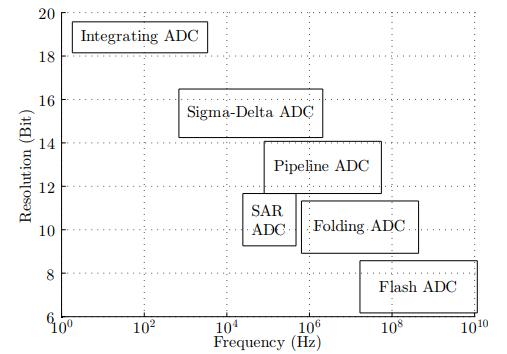
\includegraphics[scale = 0.7]{images/compare_adc.png}
\caption{Bandwidth and resolution specifications of different ADC architecture}
\label{comp_asdc}
\end{figure}

However the design of $\Delta\Sigma$ is not a easy task, as it relies on analog design techniques as well as advanced filtering and signal  processing techniques. To find a good architecture depends on proper modelling of the behaviour of the converter. 

\section{Thesis Contribution}
This thesis aims at showing the design and implementation of a $\Delta\Sigma$ modulator based on the feasibility study done in Autumn. The main objective is to achieve approximately 16 bits resolution and manage to sample it at 10MHz. The modulator was designed using 180nm complementary-metal-oxide-semiconductor (CMOS) process technology with 1.8V of supply voltage. The modulator implemented is a third order discrete time modulator which uses three low pass filters, latched comparator acting as a 1-bit quantizer and a 1-bit feedback digital-to-analog (DAC) to obtain the desired resolution. 

Figure \ref{intro_design_flow} depict the design flow of the $\Delta\Sigma$ modulator. It can be seen that a higher level define specification for a lower level. A bottom-up approach was used to verify the system i.e. starting with verifying from transistor-level and working up to system-level. The work can be divided into three stages, as described below.  



\begin{figure}[H]
\centering
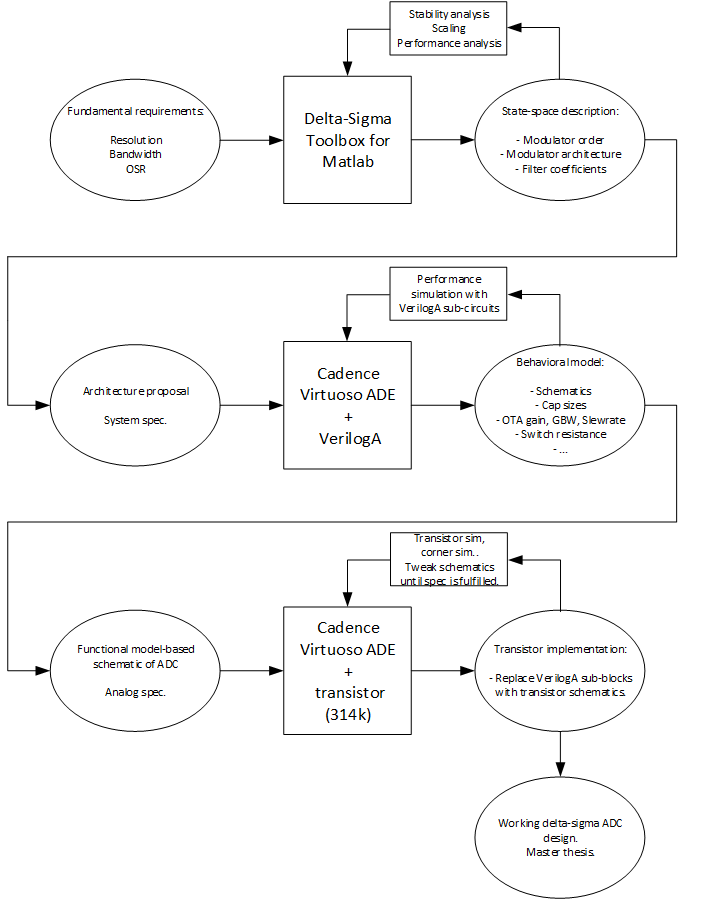
\includegraphics[scale = 0.6]{images/design_slow.png}
\caption{Design flow of the $\Delta\Sigma$ modulator}
\label{intro_design_flow}
\end{figure}

\textbf{The model was first synthesized using Richard. Schreier’s $\Delta\Sigma$ toolbox in MatLab\cite{tool}} based on the fundamental requirements, such as resolution, bandwidth and OSR. The results from the toolbox were used to derive a state description based on the modulator order, filter coefficients, number of bits of the quantizer and loop topology.  
\chapter{Background theory}\label{Background_theory}

\section{ADC Converters Fundamentals }\label{fundamentals}

The structure of an typical ADC is shown in the figure \ref{fig:adc_block}. It consists of four main blocks: an anti aliasing filter(AAF), a sample and hold circuit(S/H), a quantizer and a digital filter(decimator).
\begin{figure}[h]
\centering
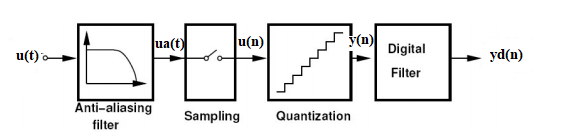
\includegraphics[scale=0.9]{images/adc_block.png}
\caption{Block diagram of a an ADC}
\label{fig:adc_block}
\end{figure}

The AAF is placed in front of the S/H circuit to remove spectral components higher than the bandwidth $\mid\frac{f_s}{2}\mid$ from the input signal $u(t)$, where $f_s$ is the sampling frequency. Thus by band-limiting the signal, it makes sure that the S/H circuit won't fold unwanted high spectral components into the band of interest. Despite being an essential block of the converters, it has to be implemented off-chip and not integrated in a ADC at a SoC-system, due to the large component values needed to realize it.  

After the signal has been conditioned to a band, the AAF's output $u_a(t)$ is sampled by the S/H circuit at the sampling frequency $f_s$. The output of the circuit will be $u(n) = u_a(nT_s)$, where $T_s$ is the sampling period($\frac{1}{f_s}$), and n is an integer in the range of 0 and the total number of samples. The next stage of the conversion process is done by the quantizer. It takes a continuous values of the sample data $u(n)$, and maps them onto a finite number of discrete values/levels. It will introduce a distinction between the mapped values and the actual analog value. This distinction is often called the quantization error($\epsilon_Q$) that is often referred to as the quantization noise of the ADC. If we assume that the quantizer's input signal $u(n)$ varies quite rapidly, then we approximate the quantizer noise to a uniformly distributed additive white noise. Hence we usually choose to model the quantizer noise as white noise with the average power given by the following expression: 

\begin{equation}
    P_E = \frac{\Delta^2}{12},
\end{equation}

where 

\begin{equation}
    \Delta = \frac{V_{FS}}{k},
\end{equation}

$V_{FS}$ is the full-scale of the quantizer, while $k$ is the number levels the quantizer consists of. Meaning if we have a N-bit quantizer, then the number of levels is given by $k = 2^N$. 

The output signal $y(n)$ of the quantizer is a digital pulse train that gets sent to the digital filter. The digital filter performs low-pass filtering and down-sampling on the signal $y(n)$ to eliminate out of band noise above the bandwidth $\frac{f_s}{2}$, and providing an output with Nyquist rate with a bit width corresponding to the ADC's resolution. 

\section{Performance metrics}

There are many metrics used to determine the performance of an ADC as shown in \cite{Allen}, \cite{Johns}, \cite{Razavi}, \cite{Barker}, \cite{Malo} and \cite{Plass}. We will look at those which are most useful to measure the performance of a $\Delta\Sigma$ modulator. These are used to analyze the output spectrum of the modulator. For example we can obtain metrics such as SNR, SNDR, DR and ENOB by analyzing outputs as depicted in figure \ref{fig:metrics} for a determined input power. 

\subsection{Resolution}
Resolution of a converter is defined as the distinct number of analog levels corresponding to the different digital words. Thus, if the ADC has a N-bit resolution, the converter can resolve $2^N$ distinct analog levels.

\subsection{Dynamic range (DR)}
Dynamic range of an ADC is defined as the range of amplitudes the ADC can effectively resolve. The ADC can overload if the signal is too large, and can get lost in the quantization noise if it too small. It can be defined in two ways. One is the ratio of the full scale value to the smallest difference it can resolve i.e. $V_{LSB}$

\begin{equation}
    DR = 6.02N.
\end{equation}

The other definition is the power of the input signal where the SNR (or the SNDR) is $0dB$. 

\subsection{Signal-to-noise ratio (SNR)}
Signal-to-noise ratio is the ratio between the signal power and the total noise power at the output. When the case is only quantization noise, it is called signal-to-quantization-noise ratio(SQNR). 

\subsection{Signal-to-noise-distortion ratio (SNDR)}
SNDR is the ratio of the signal power to the total noise and the harmonic power at the output. The parameter is also called signal-to-noise and distortion ratio(SINAD).  

\subsection{Spurious free dynamic range (SFDR)}
SFDR is defined as the ratio between the RMS value of the input sine wave for an ADC and the RMS value of the peak spur(the strongest harmonic component power) observed in the frequency domain. Some communication application require maximizing the dynamic range of the converter, here SFDR is an important parameter. 

\subsection{Total harmonic distortion (THD)}
THD is defined  as the ratio between the sum of the powers of the harmonic frequencies inside the signal bandwidth and the power of the fundamental frequency. Thus the definition can be expressed as:
\begin{equation}
    THD = \frac{\sum Harmonic frequencies}{Fundamental frequency} = \sqrt{\frac{V_2^2 + V_3^2 + .. +}{V_1^2}}
\end{equation}

\subsection{Effective number of bits (ENOB)}
This metric gives actual number of bits for a given SNDR or SINAD. It is defined by the following equation:

\begin{equation}
    ENOB = \frac{SNDR - 1.76}{6.02}
\end{equation}

\subsection{Overload level}
It is the maximum level of input amplitude for which the system can still operate correctly. 
\begin{figure}[ht]
\centering
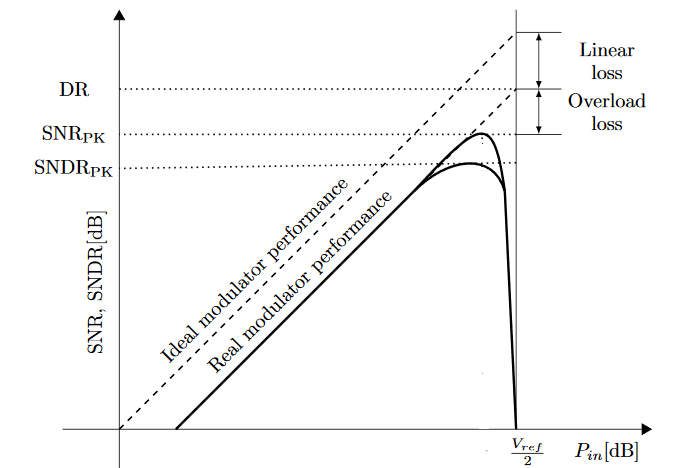
\includegraphics[scale=0.5]{images/metrics_snr.png}
\caption{Typical SNR vs. Input power}
\label{fig:metrics}
\end{figure}

\section{Classification of data converters}
Which category the data converters is placed in is influenced by the sampling frequency used for the conversion process. Broadly speaking the data converters can be classified into two categories; Nyquist-rate -and oversampling converters\cite{Ovi}.  

\subsection{Nyquist-rate converters}
The Nyquist-rate converters are based on the well known sampling theorem also known as the Nyquist theorem, which state the sampling frequency $f_s$ should be at least twice as large as the bandwidth $f_b$ in order to avoid aliasing and successfully reproduce the signal after filtering. Hence it will use an input occupying a large portion of the available bandwidth. The quantization noise in a Nyquist-rate converter is given by expression: 2.1. In Nyquist-rate converters, the sampling frequency is usually at least twice the signal bandwidth. The maximum SQNR of a Nyquist-rate converter can be obtained\cite{Richard}[Chapter 1.1], as seen in expression(2.4), where N is the number of bits.

\begin{equation}\label{no_noise_sqnr}
    SQNR_{maxNQ} = 6.02N + 1.76 dB
\end{equation}

\subsection{Oversampling converters}
In the preceding section it was mentioned that Nyquist-rate converters will use an input occupying a large potion of the available bandwidth. Oversampling converters on the other hand only occupy a small portion of the bandwidth, thus spreading the quantization noise over a wider frequency range as depicted in figure \ref{fig:oversample}. This causes the quantization noise to be reduced.  

\begin{figure}[h]
\centering
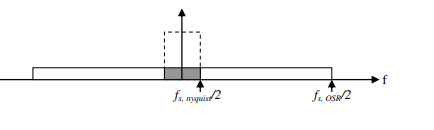
\includegraphics[scale=1]{images/oversample.png}
\caption{Quantization noise spectrum of a Nyquist-rate and a oversampling converter}
\label{fig:oversample}
\end{figure}

To be able to operate in such small portion of the bandwidth, the oversampling converters have to sample the input signal in a much higher rate than the Nyquist-rate converters. This rate is given by the oversampling ratio (OSR) which is defined as,

\begin{equation}
    OSR = \frac{f_s}{2f_b}
\end{equation}

To establish the advantage of oversampling converters compared to Nyquist-rate converters, we can look at the maximum SQNR for a oversampling converter. It can be calculated for oversampling converters\cite{Johns}[Ch 18.3], as seen in expression \ref{max_sqnr}, where N is the number of bits.


\begin{equation}\label{max_sqnr}
    SQNR_{maxOS} = 6.02N + 1.76 + 10\log_{10}(OSR) dB
\end{equation}

If we compare equation \ref{max_sqnr} with equation \ref{no_noise_sqnr}, we can see that the oversampling rate ADC can achieve the same SQNR performance as a Nyquist-rate ADC with fewer bits. Further it can be seen that for every doubling of OSR improves the SQNR with $3 dB$, or ENOB by $0.5bits/octave$. 

Another advantage of using oversampling ADCs is that the specifications of the AAF are relaxed, because the signal bandwidth is smaller than $\frac{f_s}{2}$. As shown in figure \ref{fig:AAF}, the spectral components higher than the bandwidth $f_b$ in a oversampling converter are more separated than in a Nyquist-rate converter. 

\begin{figure}
\centering
\begin{subfigure}[b]{0.35\textwidth}
   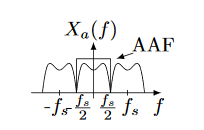
\includegraphics[width=1\linewidth]{images/nyquist_aaf.png}
   \caption{Anti aliasing filter for Nyquist-rate converter}
   \label{fig:AAf_NQ} 
\end{subfigure}

\begin{subfigure}[b]{0.55\textwidth}
   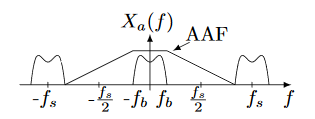
\includegraphics[width=1\linewidth]{images/over_aaf.png}
   \caption{Anti aliasing filter for Oversampling converter}
   \label{fig:AAF_OV}
\end{subfigure}

\caption{Anti aliasing filter for Nyquist-rate and Oversampling converters}
\label{fig:AAF}
\end{figure}

\section{Noise-shaping ADC}
To get a better understanding of noise-shaping, we have to first look at the $\Delta\Sigma$ modulator. The structure of typical $\Delta\Sigma$ ADC is shown in figure \ref{fig:delta_block}, which consists of four main blocks: a AAF, a S/H circuit, a $\Delta\Sigma$ modulator and a decimator. The AAF, S/H circuit and the decimator operates as explained in section \ref{fundamentals}.

\begin{figure}[h]
\centering
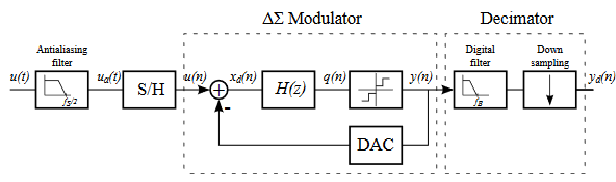
\includegraphics[scale=0.75]{images/delta_sigma_block.png}
\caption{Block diagram of a discrete-time (DT) $\Delta\Sigma$ ADC\cite{deltapic}}
\label{fig:delta_block}
\end{figure}

Even though all four blocks are essential to the ADC, our main focus for this thesis is the $\Delta\Sigma$ modulator. As shown from the figure \ref{fig:delta_block}, the $\Delta\Sigma$ modulator consists of a loop filter ($H(z)$) along with an internal quantizer and a DAC, which together makes a negative feedback loop. The basic operation of the modulator is to compare the input signal with an estimate of the output data and quantizing this difference. This structure is advantageous for oversampling signals since the amplitude of the subtracted signal $x_d(n)$ is smaller than for the input signal $u(n)$. By having a loop filter with a very high gain in the signal band, the in-band quantization noise is strongly attenuated by the feedback loop. The input signal will nearly pass unaffected through to the output. This process is known as \textit{noise-shaping}.

\section{First order $\Delta\Sigma$ modulator}\label{first_order}
To get the basic understanding in how this system works, a linear model of the $\Delta\Sigma$ modulator is shown in figure \ref{fig:linear}. The quantizer is replaced with its noise source \textit{e(n)} which we assume is white noise, and the DAC is replaced with a wire since we assume it is ideal. The system can be described by the transfer from each of the independent inputs: \textit{e(n)} and \textit{u(n)} to the output \textit{y(n)}. 

\begin{equation}
    Y(Z) = \frac{H(z)}{1+H(z)}U(z) + \frac{1}{1+H(z)}E(z)
\end{equation}

Here we can define signal transfer function \textit{STF} and noise transfer function \textit{NTF} as

\begin{equation}\label{stf_1}
    STF(z) = \frac{H(z)}{1+H(z)}U(z)
\end{equation}

and

\begin{equation}\label{ntf_1}
    NTF(z) = \frac{1}{1+H(z)}E(z)
\end{equation}

As mentioned the loop filter \textit{H(z)} has to have high gain in-band, while it may decrease outside. A commonly used filter is the delaying discrete time integrator

\begin{equation}\label{Hz}
    H(z) = \frac{z^{-1}}{1-z^{-1}}
\end{equation}

By inserting equation \ref{Hz} onto \ref{stf_1} and \ref{ntf_1}, we get

\begin{equation}\label{stf_2}
    STF(z) = \frac{\frac{z^{-1}}{1-z^{-1}}}{1 + \frac{z^{-1}}{1-z^{-1}}} = z^{-1}
\end{equation}

and

\begin{equation}\label{ntf_2}
    NTF(z) = \frac{1}{1 + \frac{z^{-1}}{1 - z^{-1}}} = 1 - z^{-1}
\end{equation}

\begin{figure}[h]
\centering
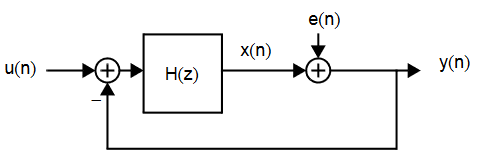
\includegraphics[scale=0.8]{images/linear_delta.png}
\caption{Linear model of $\Delta\Sigma$ modulator with inclusion of quantization noise \cite{Johns}}
\label{fig:linear}
\end{figure}

We can see from equation \ref{ntf_2} that the NTF is a high-pass filter. Therefore the in-band noise that resides on the lower frequency will be attenuated, and we can see the noise-shaping feature of the $\Delta\Sigma$ modulator. The STF \ref{stf_2} becomes a simple unit delay. This is seen as first order $\Delta\Sigma$ modulator, and the maximum SQNR is given in \cite[Ch.18.2.2]{Johns}

\begin{equation}\label{SQNR_noise}
  SQNR_{max} = 6.02N + 1.76 - 5.17 + 30log_{10}(OSR)  
\end{equation}

From equation \ref{SQNR_noise}, it can be noted that for every doubling of OSR, the SQNR improves with 9dB or ENOB with 1.5bits/octave. Compared with oversampling with no noise-shaping expression \ref{no_noise_sqnr}, we can see that the improvement is three times as good. 

In the next chapter while exploring the different aspects of the $\Delta\Sigma$ modulator, we will see how increasing the order of the loop filter H(z), can further improve the noise-shaping and thereby improve the $SQNR_{max}$. 
\chapter{Proposed Architecture}\label{architecture}

The $\Delta\Sigma$ modulator was first introduced by Inose, Yasuda and Murakami in 1962 \cite{first_delta}. Since then many modifications to the architecture have been proposed to improve its performance. There are four main aspects of the architecture where one can modify it: time-domain, order of loop filter, topology and the number of bits of the quantizer. In this chapter we will review the different alternatives for an architecture with respect to the four aspects. To ease the discussion, we will mainly focus on single-loop architectures, since it will be integrated in a microcontroller and a simple architecture is desired. By designing a more complex system, we will only end up with an over-engineered proposal. 

A small discussion of the proposed architecture found in the feasibility study will be presented in the last section. The bases for the discussion is based on the well known book; \textit{Understanding Delta-Sigma Data Converters}\cite{Richard}. Additionally a discussion around different topology of OTAs, and the choice between single ended and fully differential output will be discussed.  

\section{Order of loop filter}

The expression of maximum SQNR for first order $\Delta\Sigma$ modulator \ref{no_noise_sqnr} showed that for every doubling of the OSR yielded in increasing the SQNR with 9dB or ENOB with 1.5bits/octave. To be able to achieve a higher resolution i.e. higher ENOB, a larger OSR has to be used. The drawback with using a large OSR is that it requires large $f_s/f_b$, which can be hard or impossible to realize. 

An obvious way to increase ENOB of the $\Delta\Sigma$ modulator is to use a high-order loop-filter. It can done by replacing the integrator in Fig. \ref{fig:linear} with \textit{L} number of integrator consecutively, where \textit{L} corresponds to the order of the loop-filter. The NTF can then be given by

\begin{equation}
    NTF = (1-z^{-1})^L
\end{equation}

In figures \ref{fig:SQNR} and \ref{fig:ENOB} it is shown how much OSR one need to achieve ideal SQNR and ENOB respectively, for different order of integrator. It can be observed to achieve 16 bit resolution, modulators on the order of 2 and 3 is sufficient. It can also be observed that the modulator with order 2 needs much larger OSR, which can cause problems with $f_s/f_b$.

\begin{figure}
\begin{minipage}[c]{0.5\linewidth}
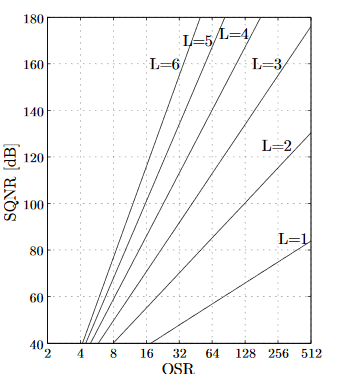
\includegraphics[width=\linewidth]{images/OSR_vs_SQNR.png}
\caption{Ideal SQNR vs OSR\cite{SQNR}}
\label{fig:SQNR}
\end{minipage}
\hfill
\begin{minipage}[c]{0.5\linewidth}%
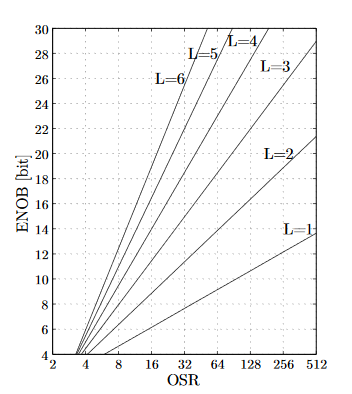
\includegraphics[width=\linewidth]{images/ENOB_vs_SQNR.png}
\caption{Ideal ENOB vs OSR\cite{SQNR}}
\label{fig:ENOB}
\end{minipage}%
\end{figure}

Instability is an issue higher-order filters are struggling with. For first and second order filters, this is not a problem, but as the order of the filters gets bigger, the out-of-band gain(OBG) of the modulator gets more aggressive. The high OBG can cause overloading of the quantizer which can make the modulator unstable. 

One can achieve stable operation by letting the input level be less or equal to the fullscale of the first feedback DAC. For high-order single-bit $\Delta\Sigma$ modulators this input range should be a few dB below the DAC fullscale\cite[Chapter 4.2]{Richard}. A rule of thumb to check if a high-order single bit $\Delta\Sigma$ modulator is stable is to use Lee's Criterion\cite{Lee}:

\begin{equation}
    |NTF_{max}| \leq 1.5
\end{equation}

where $|NTF_{max}|$ is the maximum magnitude over all frequency. Even when the criteria is fulfilled, there is a change the system will become unstable, because of the quantizer in the loop can turn the system into non-linear one\cite{Richard}. 

\section{Topologies}
The alternatives to implement a $\Delta\Sigma$ modulators can be categorized into two categories: a single-loop or a cascade architecture. The first one refer to the use of only one quantizer, as seen in the section \ref{first_order}. The other one refer to multi-stage noise-shaping (MASH) modulator which is a popular structure that eases the stability problems associated with high-order modulators. Even though it has its advantages, we will not look into MASH modulators. The single-loop architectures are simpler to design and they are able to achieve the specifications given in chapter 1 at a $\Delta\Sigma$ order of 2 and 3. We will now look at the two most used single-loop architectures; feedforward and feedback topologies. 

\subsection{Feedback topology}
The figure \ref{fig:back} depict an example of $3^{rd}$ order feedback topology. The STF and NTF for this topology is given by
\begin{equation}
    STF = \frac{b_1c_1c_2c_3H^3(z)}{1 + a_3c_3H(z) + a_2c_2c_3H^2(z) + a_1c_1c_2c_3H^3(z)}
\end{equation}

and
\begin{equation}
    NTF = \frac{1}{1 + a_3c_3H(z) + a_2c_2c_3H^2(z) + a_1c_1c_2c_3H^3(z)}
\end{equation}

Here the forward coefficients ($c_1, c_2$ and $c_3$) represent the scaling or weighed of the integrators. The purpose of them is to scale the output dynamic range of the integrators. The coefficients on the feedback path ($a_2$ and $a_3$) are used to create a transfer function that gives a noise-shaping, while the feedback coefficient $a_1$ ensure that the output from the quantizer tracks the input.

One of the major drawbacks with this topology is that the output swings of the integrators tends to get big, which means that the the op-amp requirement has to be increased to avoid overloading. Furthermore the forward coefficients $c_i$ has to become smaller in order to scale down the swing. The drawback on having small coefficients is that the area to maintain the same capacitor noise gets bigger, which leads to more power to charge capacitor. Another drawback is that unlike the feedforward-path, the output of the first integrator contains some amount of the input amplitude. This leads to higher swing capabilities, which again leads to a more power-consuming system.   

\begin{figure}[H]
\centering
\begin{subfigure}[b]{0.85\textwidth}
   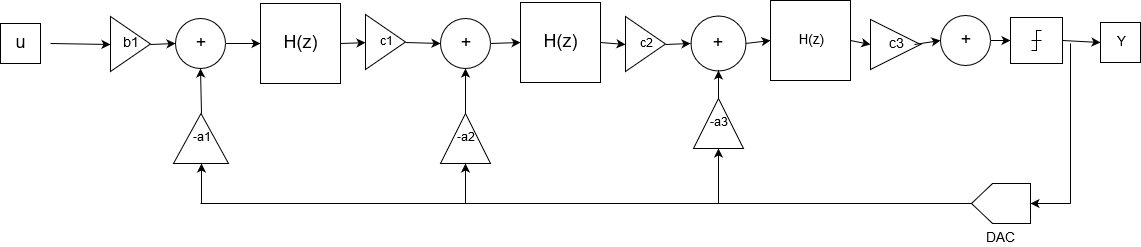
\includegraphics[width=\textwidth]{images/feedback.png}
   \caption{Feedback}
   \label{fig:back} 
\end{subfigure}

\begin{subfigure}[b]{0.85\textwidth}
   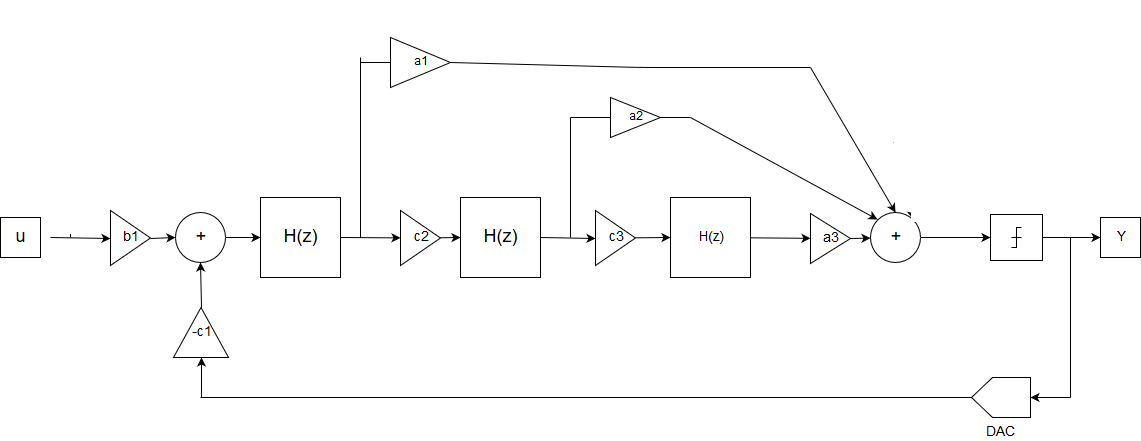
\includegraphics[width=\textwidth]{images/feedforward_no.png}
   \caption{Feedforward}
   \label{fig:forward}
\end{subfigure}

\caption{$3^{rd}$ order loop realization structures for feedforward and feedback}
\end{figure}

\subsection{Feedforward topology}
An example on the $3^{rd}$ order feedforward topology is depicted in figure \ref{fig:forward}. Unlike the feedback topology, this one has only one feedback from the quantized output. The coefficients ($a_1, a_2$ and $a_3$) are forwarded to the output, where their weight is added to the quantizer input. The STF and NTF are then given respectively,

\begin{equation}
    STF = \frac{b_1(a_1H(z) + c_2a_2H^2(z) + c_2c_3a_3H^3(z))}{1 + b_1(a_1H(z) + c_2a_2H^2(z) + c_2c_3a_3H^3(z))}
\end{equation}

\begin{equation}
    NTF = \frac{1}{1 + b_1(a_1H(z) + c_2a_2H^2(z) + c_2c_3H^3(z))}
\end{equation}

By moving the coefficients to the summation node in front of quantizer, the signal presented at integrators output will be significantly lower than at the feedback topology. This leads to lesser swings and scaling, which means that the op-amp requirement can be relaxed, which leads to less power consumption. However one should be aware of operating on input amplitude near the reference voltage ($V_{ref}$), as this will drive the modulator to instability. The feedforward topology can further be improved by having a feedfoward path from input signal to the summation node in front of the quantizer, as shown in Fig. \ref{fig:input}. This means that the integrators do not process the input signal, only quantization noise $U$, and this leads to low distortion\cite[Ch.4.4.2]{Richard}, further relaxing the requirement for the integrator's op-amp. One thing to notice is that having fewer internal feedback DACs reduce the power dissipation significantly. 

\begin{figure}\label{final_top}
\centering
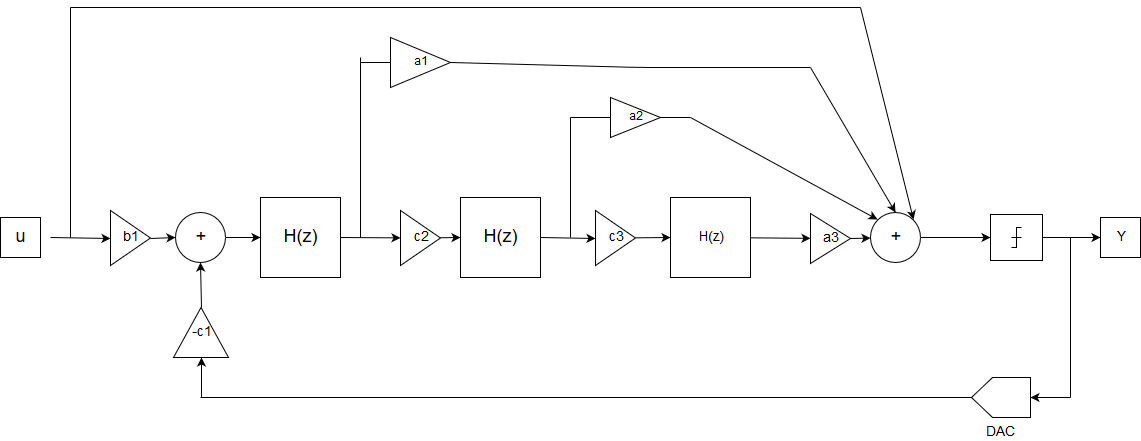
\includegraphics[scale=0.35]{images/feedforward.png}
\caption{$3^{rd}$ order feedforward topology with input signal forwarded to summation node}
\label{fig:input}
\end{figure}

\section{Time-domain}
The $\Delta\Sigma$ modulator can operate in a discrete-time domain (DT) or in the continuous-time domain(CT)\cite{Richard}. We have already seen how DT modulator operates in chapter \ref{Background_theory}. Figure \ref{fig:cont} illustrates a simple first order continuous time (CT) $\Delta\Sigma$ modulator. Unlike the DT $\Delta\Sigma$ modulator, the input signal and the integrator are continuous and the sampling occurs only before quantization. The STF and NTF for CT modulators has the same as the DT one.    

The main difference, is the way they are implemented. The DT $\Delta\Sigma$ modulators employ switched-capacitor (SC) integrators while CT systems use active-RC integrators in the modulators. To choose the right domain for a application, one has to look at the advantages and disadvantages of associated with each option.

Switched-capacitor has the perk of taking advantages on fine-line very large scale of integration (VLSI) capabilities by eliminating the need to use physical resistors. Furthermore capacitors have high linearity, which is difficult to achieve with on-chip resistors in a standard CMOS process. In addition, the resistors in CT integrators can not afford to get too big as it can affect the thermal noise by increasing it, but having small resistors can increase the feedback capacitors, if one want to preserve the same settling time. 

The accuracy of SC integrators is good, since the matching between capacitors are much better than matching between capacitor and resistors. Hence, the accuracy of the CT integrators will be inferior to SC integrators\cite[Ch.6.6]{Richard}. Another advantage is that the SC systems is less sensitive to clock jitter.

The CT modulators is attractive to high-speed applications as it can achieve very high OSR and is four times faster than DT modulators\cite{Richard}. The DT modulators are limited by the achievable bandwidth of the opamps. Instead of having AAF outside the modulator as the DT modulator, the CT modulator has implicit AAF, since the sampling happens outside the loop-filter which is low-pass. The elimination of this filter can lead to power savings for the receiver.

\begin{figure}[H]
\centering
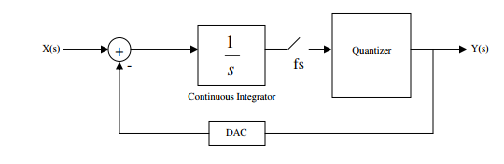
\includegraphics[scale=0.9]{images/cont.png}
\caption{Linear model of CT first order $\Delta\Sigma$ modulator}
\label{fig:cont}
\end{figure}

\section{Single-bit vs multi-bit quantizer}
For a full-scale, the quantization error is reduced by 6dB for every bit added to the resolution of the quantizer\cite[Ch.6]{Richard}. Meaning that the SQNR will increase with this amount leading to a more stable operation. This is especially good for modulators of high order. Also the feedback loop becomes more linear, consequently allowing us to choose NTF more aggressively. Hence even better SQNR can be obtained, and larger input signals can be used. This and more advantages makes multi-bit quantizer attractive to use. However the errors introduced by DACs are not attenuated as quantization errors. Since the DAC's output goes to the input signal, the errors will get injected with the signal. As the linearity of the modulator is deepened on the linearity of the DAC. Multi-bit quantizer struggles with being linear, and need costly corrections techniques to keep up with the high linearity demand. This is not a problem for single-bit quantizer, since the DAC is inherently linear.

Another advantage with multi-bit quantizer is that it does not require large OSR as single-bit. Meaning the requirement for the bandwidth of a opamp can be relaxed. However adding more bits leads to a bigger power dissipation, making single-bit quantizer more attractive for applications that demand low power.

\section{Choosing architecture}
The requirement of the modulator is to achieve 16-bit resolution. Three things were considered in choosing the right architecture: area, power and requirement for the system. The final architecture that was selected was a discrete-time third-order single-bit single-loop feedforward architecture with the input forwarded into the summation node, as shown in Fig. \ref{fig:input}.

The choice of modulator order was between second and third order, which both satisfied the specification with OSRs: 256 and 128 respectively. As the mentioned in section 3.1, the high OSR of second order can cause the ratio between the sampling frequency and the bandwidth to become large. Furthermore, the high OSR also leads to stricter requirement for the opamp. The third order modulator takes bigger area and has stricter stability requirement, but having a relax requirement seemed more desirable. However the OSR was chosen to be 170, as we want the theoretical SQNR to be 10-20dB more than the desired SNR in order to allow degradation in SQNR due circuits non-idealities and leave as much of the noise budget for thermal noise\cite[Ch.9.2]{Richard}.

The feedforward topology was chosen because it gives the best $SNR_{peak}$. Moreover implementing feedback means that the power dispassion gets significantly larger, since the DAC's output is connected to the output of the integrators. One thing to remember is to have input amplitude a few dB under $V_{ref}$. Since $V_{ref}$ was chosen to be 1V, the input amplitude was chosen to be 0.5.

Finally, DT-time single-bit architecture is the most suitable for the application, since it is easier to implement an SC integrator, and it is the best option considering noise budget and power savings. Also, with the superior linearity that follows with single-bit architecture, makes it more desirable to implement considering the cost in power and complexity it will take to reach stability. The specifications for the modulator have been 
summarized in table \ref{spec}.

% Please add the following required packages to your document preamble:
% \usepackage{booktabs}
\begin{table}[H]
\centering
\caption{Specification for ,odulator}
\label{spec}
\begin{tabular}{@{}ll@{}}
\toprule
Parameter       & Value        \\ \midrule
Resolution      & 16           \\
Fs              & 10MHz        \\
OSR             & 170          \\
Vdd             & 1.8V         \\
$V_{ref}$          & 1V           \\
Input amplitude & 0.5          \\
Order           & 3            \\
Topology        & Feed forward \\
Domain          & DT           \\
Quantizer level & 2            \\ \bottomrule
\end{tabular}
\end{table}
\chapter{Specification of the design}\label{specifiation}
In the feasibility study a set of specifications were obtained using behavioural modeling. In this chapter a small discussion of the results will be presented with additional specifications needed to implement the circuit design.

The specifications can be divided into two categories as listed below. 
\begin{itemize}


\item \textbf{Requirements for the integrators}: The requirement for the total noise was derived in the feasibility study to find the optimal size for the capacitors used by the integrators and the summing node. In the feasibility study it was found out that matching requirements were needed, and with parameters given by \textit{Microchip} \cite{private}, we could calculate realizable capacitors values. In this thesis the matching requirements are the same, but the parameters are different, thus giving us a new set of capacitors values. The switch's on resistance were found after an exhaustive iteration of simulation.

\item \textbf{Requirements for the Amplifier}: After an exhaustive iteration of simulation, the specifications for the finite DC gain, GBW and slew rate were found. The output-swing and the load capacitance seen from each output of the OTAs is also presented here. 
\end{itemize}

\section{Sizing of Capacitors}
The proposed architecture was a discrete-time third-order single-bit single-loop feedforward $\Delta\Sigma$ modulator, as shown in figure \ref{fig:input}. The transfer function for the non-inverting integrators is given by,

\begin{equation}\label{transfer_integrator}
    H(z) = \frac{C_s}{C_i}\cdot \frac{z^{-1}}{1 - z^{-1}}
\end{equation}

where $C_s$ is the sampling capacitor and $C_i$ is the integrating capacitor. The coefficients $b_1, c_1$ and $c_2$ describe the relationship between these capacitors for integrator 1, 2 and 3 respectively. For instance the capacitors' relationship in integrator 1 can be described by

\begin{equation}
    b_1 = \frac{C_s}{C_i}
\end{equation}

The feedforward coefficients $a_1, a_2$ and $a_3$ describe the parallel network of capacitors in the summation circuit shown in appendix ??

The coefficients found in the feasibility study are given in table \ref{scale}.

\begin{table}[h]
\centering
\caption{Coefficients}
\label{scale}
\begin{tabular}{|l|l|l|}
\hline
Coefficients  &      \\ \hline
$b_1$         & 0.32 \\ \hline
$c_2$         & 0.69 \\ \hline
$c_3$         & 0.16 \\ \hline
$a_1$         & 2.56 \\ \hline
$a_2$         & 1.32 \\ \hline
$a_3$         & 1.27 \\ \hline
\end{tabular}
\end{table}

The matching requirements is given in table \ref{match}.

\begin{table}[h!]
\centering
\caption{Matching requirement}
\label{match}
\begin{tabular}{|l|l|}
\hline
Coefficients & Matching \\ \hline
$a_1$           & $\pm4\%$        \\ \hline
$a_2$           & $\pm4\%$        \\ \hline
$a_3$           & $\pm4\%$        \\ \hline
$c_2$           & $\pm2\%$      \\ \hline
$c_3$           & $\pm1\%$        \\ \hline
\end{tabular}
\end{table}

Using the coefficients with the matching requirements and parameters given by \textit{Microchip}, the final values can be computed. The capacitors that realize  $a_1, a_2$ and $a_3$ are matched to the same reference (the feed-forward capacitor). Thus, the following realization of the coefficients is proposed:

\begin{table}[h!]
\centering
\caption{Realizable coefficients}
\label{RC}
\begin{tabular}{|l|l|l|l|}
\hline
Coefficients & Ideal value & Fractional value & Cap realization \\ \hline
b1           & 0.32        & 542/1779         & 2.05p/6.58p     \\ \hline
a1           & 2.56        & 64/25            & 236.8fF/92.5fF \\ \hline
a2           & 1.32        & 33/25            & 122.1fF/92.5fF  \\ \hline
a3           & 1.27        & 32/25            & 118.4fF/92.5fF  \\ \hline
c2           & 0.69        & 7/10             & 76fF/106.4fF \\ \hline
c3           & 0.16        & 3/19             & 45.6fF/288.8fF   \\ \hline
\end{tabular}
\end{table}

\section{Switches' on-resistance}\label{on-resistance}
The size of the switches' on-resistance have to be specified to estimate the cost of implementing it on transistor-level. Having small on-resistance will lead to bigger area usage, and it will therefore be costly to implement. The goal in the feasibility study was to find the largest on-resistance for the integrators that will give the desired performance. The final values are summarized in table  

\begin{table}[H]
\centering
\caption{Final specification for the switches' on-resistance}
\label{spec_res}
\begin{tabular}{|l|l|l|l|l|l|}
\hline
Specifications & Integrator 1 & Integrator 2 & Integrator 3 & Summing node &    \\ \hline
Ron            & 0.9            & 1.5          & 1.6          & 1.7          & $k\Omega$ \\ \hline
\end{tabular}
\end{table}

\section{Finite DC-gain}

Finite DC-gain will give integrator leakage, which can in general be expressed as:

\begin{equation}
    H(z) = \frac{1}{z - \alpha}, \alpha = 1 - \frac{1}{A_0}
\end{equation}

This means the integrator has a DC-gain limited by opamp's open-loop gain, which again means that the DC-attenuation of the NTF is also limited. In general the cascade of opamps' gains much be much higher than the desired NTF DC-attenuation, or in other words higher than the resolution. The effect of limiting gain is shown in figure \ref{fig:DC_gain_spec}. AS seen the third order modulator has small open-loop gain, raging from 35dB to 45dB. The reason being all the NTF's zeroes will be in DC. Therefore the cascade of open-loop gains of the integrators are sufficient enough to give the desirable performance. Another advantage of having small gains is that the specifications for gain for each OTA are relaxed, thus one can easily achieve the requirement with a one stage OTA. 

\begin{figure}[H]
\centering
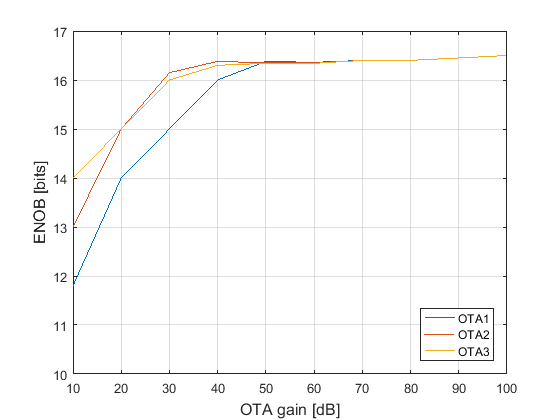
\includegraphics[scale=0.7]{images/DC_gain_spec.png}
\caption{ENOB limitation due to finite open}
\label{fig:DC_gain_spec}
\end{figure}

\section{Output swing}\label{out_put_swing}
In figure \ref{fig:output_swing} we see the output swing of integrator 1, 2 and 3. We have that for integrator 1 and 2 the output swings from 0.6 to 1.2, while for integrator 3 it swings from 0.7 to 1. This gives us voltage change ($\Delta V_{1,2}$) of 0.6 for integrator 1 and 2, and $\Delta V_3$ of 0.3 for integrator 3. It is worth mentioning that when the output voltage is closer to limits, the response is distorted.    

\begin{figure}[h]
\centering
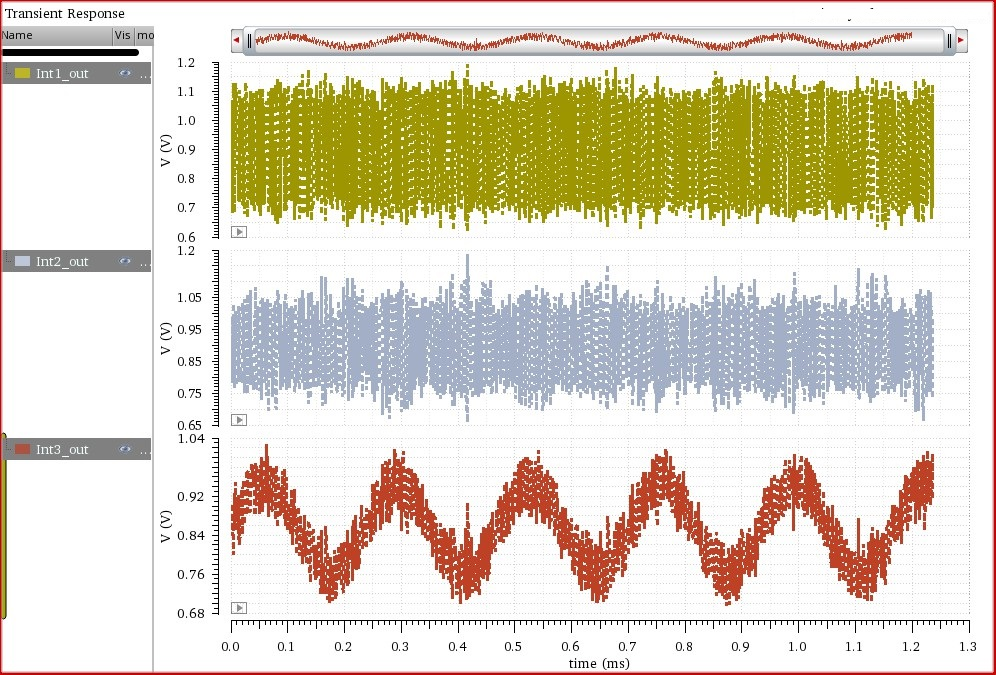
\includegraphics[scale=0.45]{images/output_swing.jpg}
\caption{Output swing of integrator 1, 2 and 3}
\label{fig:output_swing}
\end{figure}

\section{Gain-Bandwidth Product an Slew-Rate}

Finite gain-bandwidth (GBW) of the OTA will lead to incomplete linear settling as the output will not settle to its final value. This will cause the ENOB to degrade, therefore we need to find sufficient GBW to achieve the desired ENOB. The degradation of ENOB with falling GBW is shown in figure \ref{fig:GBW_spec}. It was found out the minimal GBW should be between 28MHz and 38MHz. If we choose smaller GBW, the performance will degrade rapidly. Making this specification one of the most critical.

\begin{figure}[h]
\centering
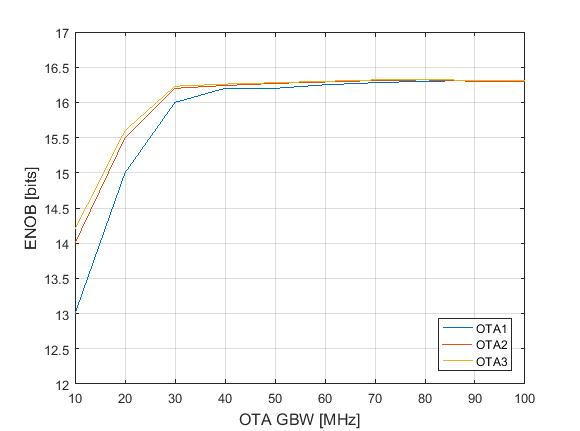
\includegraphics[scale=0.55]{images/GBW_spec.jpg}
\caption{ENOB limitation due to GBW}
\label{fig:GBW_spec}
\end{figure}

Unlike linear settling error, slewing causes non-linear settling error which degrade the ADCs linearity. The slew- rate must be high enough to avoid slewing to cause non-linear settling error. Meaning it must be high enough to settle the output in $\frac{T_s}{2}$, where $T_s$ is the sampling period. This gives us the requirement for minimum slew-rate:

\begin{equation}\label{sr}
    \frac{\Delta V}{SR} > \frac{T_s}{2}
\end{equation}

where $\Delta v$ is the output change in the integrator. We from section \ref{out_put_swing}, that the output change is 0.6 for integrator 1,2 and 0.3 for integrator 3. By performing transient analysis we found out the slew-rates given by equation \ref{sr} are not sufficient. The calculated and the final simulated values are summarized in table \ref{SR_final}.

\begin{table}[H]
\centering
\caption{Theoretical and Simulated Values of SR}
\label{SR_final}
\begin{tabular}{|l|l|l|}
\hline
Integrator & Calculated & Simulated \\ \hline
1           & 12MV/sec   & 28MV/sec  \\ \hline
2           & 12MV/sec   & 28MV/sec  \\ \hline
3           & 6MV/sec    & 28MV/sec  \\ \hline
\end{tabular}
\end{table}

\section{Load Capacitance}
To be able to design the OTAs correctly so that they function properly in the whole system, we need to find the load capacitance they see at their output. Using method introduced in \cite{load}, we can estimate what the load capacitance for each OTA will be. As an example we can compute for the first OTA. We have that.

\begin{equation}\label{cap_load}
    C_{L1} = C_{s1}||C_{i1} + C_{s2} + C_{ff1} + 0.2\dot(C_{i1} + C_{s2} + C_{ff1}) \approx 3.5p 
\end{equation}

where $C_{s1}$, $C_{i1}$ and $C_{ff1}$ are the sampling, integrating and feedforward capacitor of the first integrator. Same way we can find the load capacitance for second and third OTA, and they are $0.6p$ and $0.3p$ respectively. 

\section{Specifications of the Amplifier}
Table \ref{spec_ota} summarize the requirements for the amplifiers of integrator 1, 2 and 3. It has also been included a specification for phase margin. It has been chosen to be greater than $60^\circ$, because it allows for the fastest settling time when attempting to follow a voltage step input \cite{phase}. 

\begin{table}[H]
\centering
\caption{Specifications of the Amplifiers}
\label{spec_ota}
\begin{tabular}{|l|l|l|l|}
\hline
Parameter        & OTA1     & OTA2     & OTA3     \\ \hline
$A_O$             & $>$45dB     & $>$35dB     & $>$35dB     \\ \hline
GBW              & $>$38MHz    & $>$30MHz    & $>$28MHz    \\ \hline
SR               & $>$28MV/sec & $>$28MV/sec & $>$28MV/sec \\ \hline
Output Swing     & 0.6$<$Vout1$<$1.2 & 0.6$<$Vout2$<$1.2  & 0.7$<$Vout3$<$1         \\ \hline
Phase Margin     & $>$60$^\circ$       & $>$60$^\circ$       & $>$60$^\circ$       \\ \hline
Load Capacitance & 3.5p     & 0.6p     & 0.3p     \\ \hline
\end{tabular}
\end{table}

\section{Impact of nonidealities}

The non-ideal model of the modulator was simulated using the first three specifications given by table \ref{spec_ota}, and the capacitance summarized in table \ref{RC}. The output spectra is shown in figure \ref{fig:psd_non_ideal}, where the SNR and ENOB values are also shown. It can be noted that the main objective of achieving ENOB of 16 bits is satisfied.   

\begin{figure}[ht]
\centering
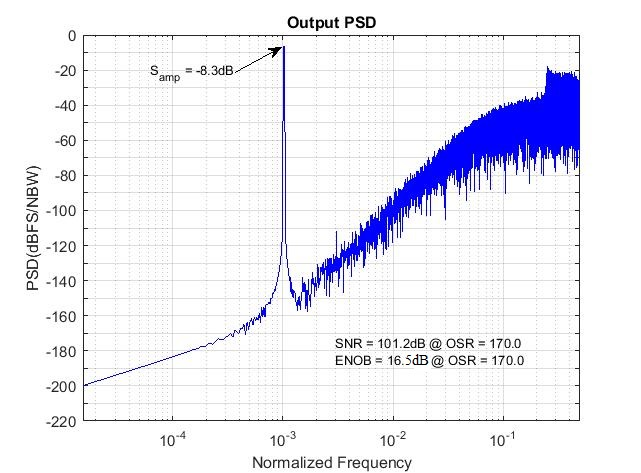
\includegraphics[scale=0.55]{images/psd_out_spec.jpg}
\caption{PSD of the output signal using non-ideal model}
\label{fig:psd_non_ideal}
\end{figure}

\chapter{Circuit Design}
This chapter describe the design methodology of implementing analog blocks used in third order $\Delta\Sigma$ modulator, and also address the issues involving the design of the modulator. 
Moreover the procedure to obtain the final transistor dimensions were based on the $gm/I_D$ methodology and on iterative simulations, since the equations used in the SPICE level 1 are not accurate. 

\section{Switched-capacitor circuits}

As discussed in chapter \ref{architecture} resistors occupy huge space in a layout and they are also the sources of noises, which makes them unattractive to use in integrated circuits. A switched capacitor circuit can be used to emulate the behaviour of a resistor by a capacitor in and out of the circuit. Figure \ref{fig:switched_cap} depict a switch-capacitor circuit, where \textit{$V_1$} and \textit{$V_2$} are two dc voltage sources. The clock periods $\phi_1$ and $\phi_2$ are a pair of overlapping clocks, which means that the capacitor $C_1$ is charged to $V_1$ and then $V_2$ during each clock period. This charge transfer is repeated every clock period with a clock period of $T_s$. Thus, the average current is given by the charge moved in one clock period\cite{Johns}:  

\begin{equation}\label{sw_res}
    I_{avg} = \frac{C_1(V_1 - V_2)}{T_s}
\end{equation}

\begin{figure}[h]
\begin{subfigure}[c]{0.4\linewidth}
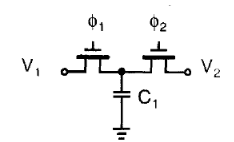
\includegraphics[width=\linewidth]{images/switched_cap_res.png}
\caption{Switched-capacitor circuit}
\label{fig:switched_cap}
\end{subfigure}
\hfill
\begin{subfigure}[c]{0.3\linewidth}
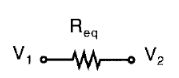
\includegraphics[width=\linewidth]{images/res.png}
\caption{Resistor equivalent}
\label{fig:resistor}
\end{subfigure}

\caption{Resistor equivalence of switched capacitor capacitor}
\end{figure}

From the equivalent resistor circuit shown in figure \ref{fig:resistor}, we have that the current through the resistor is:

\begin{equation}\label{eq}
    I = \frac{V_1-V_2}{R_{eq}}
\end{equation}

Comparing equations \ref{sw_res} and \ref{eq}, we see that the average current through the SC circuit will be equal to the resistor circuit if:

\begin{equation}
    R_{eq} = \frac{T_s}{C_1} = \frac{1}{C_1f_s}
\end{equation}

A disadvantage is that the switches are implemented using transistors, and their non-idealities can degrade the SC circuit performance. 

\section{Switched-capacitor integrators}
A differential switched-capacitor integrator circuit is shown in Fig. \ref{fig:DT_integrator}. It is known for its insensitive to parasitic capacitance of the sampling capacitor ($C_s$). The operation of the SC integrator can be explained by examining the charges on the capacitors on each clock phase. For simplicity we will only look at the top half circuit, since the bottom one has the same operation. It is assumed that the initial voltage stored in $C_f$ is zero. Switches \textit{S1} and \textit{S3} are closed during phase $\Phi_1$, while the others are closed during phase $\Phi_2$. Note that $\Phi_1$ and $\Phi_2$ are two non-overlapping phases. When \textit{S1} and \textit{S3} are closed, the input source charges the capacitor $C_s$ to a initial charge of $C_sV_{IN}$. During phase $\Phi_2$, switches \textit{S2} and \textit{S4} are closed. Thus the input is disconnected from the circuit, and the bottom plate of capacitor $C_s$ is connected to ground. Therefore the charge stored on the capacitor $C_s$ is transferred to the capacitor $C_f$. Then when phase $\Phi_1$ is active again the input voltage charge $C_s$ with a new sample. Then during phase $\Phi_2$, the charge from the new sample is transferred to the capacitor $C_f$ where it accumulates with the previous charge from the first operation. The integrator corresponds to a non-inverting one, and the transfer function is given by equation \ref{transfer_integrator}.

\begin{figure}[h]
\centering
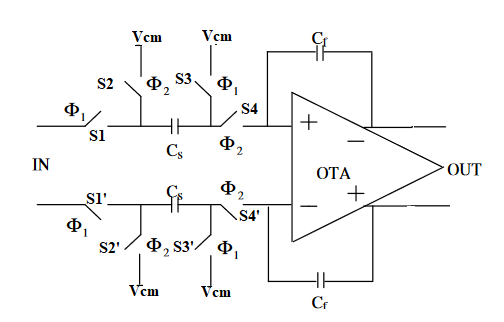
\includegraphics[scale=0.8]{images/DT_integrator.png}
\caption{Parasitic-insensitive integrator}
\label{fig:DT_integrator}
\end{figure}


\subsection{Channel charge injection and bottom-plate sampling}
Charge injection can be understood using the circuit in Fig. \ref{fig:charge_injection}. When the MOSFET switch is \textit{on} and $V_{DS}$ is small, there is a charge present in the inversion layer called channel charge $Q_{ch}$. When the MOSFET turns of, this charge is injected onto the capacitor $C_{load}$ and into $V_{in}$. Since $V_{in}$ is assumed to be a low-impedance, source driven node, the injected charge has no effect on this node. However, the charge injected onto $C_{load}$ results in a change in voltage across it, introducing an error in reading the correct input signal. 

\begin{figure}[H]
\centering
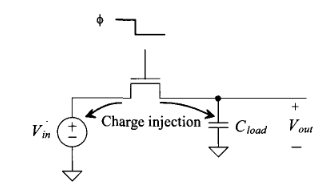
\includegraphics[scale=0.9]{images/charge_injection.png}
\caption{Charge injection in a sampling circuit}
\label{fig:charge_injection}
\end{figure}

Although charge injection mechanism is complex to characterize, many techniques have been used to minimize its effect. One being bottom-plate sampling technique\cite{Barker} which is employed to make charge injection of switches independent of the input signal. Figure \ref{fig:bottom_sampling} shows the integrator again, but now with delayed phases $\Phi_{1d}$ and $\Phi_{2d}$ with respect to phases $\Phi_1$ and $\Phi_2$ respectively. Switches \textit{S3} and \textit{S4} are turned off slightly before switches \textit{S1} and \textit{S2}, so that $C_s$ sees a high impedance. Thus, the charge injection introduced by switches \textit{S1} and \textit{S3} flows towards the low-impedance source node and almost no charge is accumulated onto sampling capacitor $C_s$.

\begin{figure}[ht]
\centering
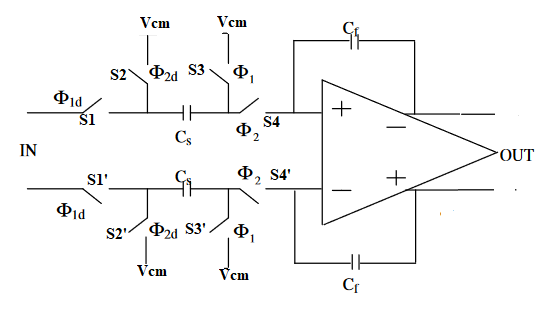
\includegraphics[scale=0.7]{images/DT_integrator_delayed.png}
\caption{Integrator with bottom-sampling technique}
\label{fig:bottom_sampling}
\end{figure}

\subsection{Correlated double sampling}

Correlated double sampling (CDS) technique was first introduced by White, Lampe, Biaha and Mack \cite{cds} as a technique for removal of switching transients and elimination of the Nyquist noise. What is more interesting is that it can be used to attenuate errors due to flicker noise $1/f$, finite offset voltage and finite opamp gain \cite{corr}. The technique is only used on the first integrator since the noise contribution is most critical in it. The noise contribution in the subsequent integrators are small, since the noise will be significantly attenuated as discussed in the feasibility study. 

We will use a simple SC integrator depicted in Fig. \ref{fig:cds} to illustrate how the CDS technique works. During $\phi_1$, the capacitor $C_2'$ samples the input offset voltage of the opamp. Then $C_2'$ is connected in series with the opamp's inverting input during phase $\phi_2$. The error from the opamp gets subtracted from the one stored in $C_2'$, thus minimizing it. For a differential SC integrator a symmetrical circuit of the one shown in \ref{fig:cds} is connected to the non-inverting input.  

\begin{figure}[ht]
\centering
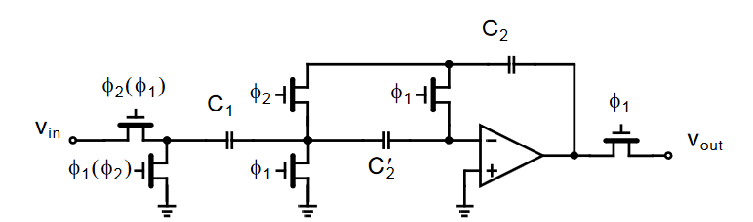
\includegraphics[width=\textwidth]{images/cds.png}
\caption{Simple SC integrator using CDS technique \cite{Johns} }
\label{fig:cds}
\end{figure}

Another thing to note is that CDS will square the effective gain to the opamp due the extra capacitors, so the open-loop gain of the OTA for integrator will get relaxed, as seen in table \ref{spec_ota}, but at the expanse of bigger area. The resulting schematic of integrator 1 is shown in Fig. \ref{app:integrator_1}, and the schematic used for the other two integrators is shown in Fig. \ref{app:integrator_rest} in appendix \ref{app:cicuits}. 


\section{Switches}
Sampling switches is one of the most fundamentals analog blocks of ADC operating on discrete-time. An ideal switch is just short circuit when it is on and an open circuit when it is off. In other words when the switch is on there should be zero resistance, and when the switch is off there should be an infinity resistance. But as discussed in section \ref{on-resistance}, these values are not feasible. Therefore designing the switches with adequate on-resistances without degrading the performance is a crucial part in the design of integrated circuits (ICs). 

The commonly used switch implementations are: a NMOS transistor, a PMOS transistor or a transmission gate (TG). The on-resistance of a MOSFET depends on the input signal, as given in \cite{Allen}, and rewritten in expression \ref{R_on}:

\begin{equation}\label{R_on}
    R_{on} = \frac{1}{\mu C_{ox}\frac{W}{L}(V_{GS} - V_T)}
\end{equation}

Where the mobility $\mu$ is different depending on if we look at NMOS or PMOS transistor. We have that the time-constant increases for more positive NMOS or negative PMOS inputs. Designing a switch with large enough input swing capability is a challenge in low-voltage application. The reason being that as the technology scales, the supply voltage scales down much faster than the threshold voltage of a transistor. For a NMOS the operation is restricted to a input swing lower than $V_{DD} - V_{thn}$, and for PMOS the swing must be greater than $V_{thp}$. 

Transmission gate is a technique that can be used to accommodate greater swings \cite{Barker}. It consists of a PMOS in parallel with a NMOS transistor as shown in Fig. \ref{fig:TG_switch}. The disadvantage of such switch is to have extra circuit to implement the complementary clocks, but it is a small price to pay for an improvement as good as rail-to.rail swing across the switch.     

\begin{figure}[h]
\centering
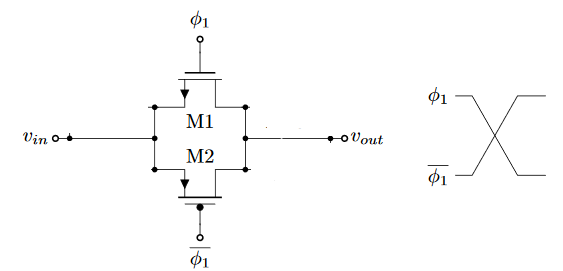
\includegraphics[scale=0.7]{images/TG_switch.png}
\caption{Circuit implementation of a TG switch}
\label{fig:TG_switch}
\end{figure}

After choosing the topology for the switch, the dimensions of the transistors were found. Using equation \ref{R_on} and Fig. \ref{fig:TG_switch} we get that: $V_{GS} = \phi_1 - v_{in}$, where $\phi_1$ is $V_{DD}=1.8V$ when it is on and 0V when it is off. After completing a simulation it was found out that the on-resistance for the resistors were too high. We cannot change the swing of the input voltage $V_{in}$, since it is given by the system. The options were either to increase the dimension $\frac{W}{L}$ or increase the gate voltage $\phi$ when it is high. Since we want to keep the dimensions as small as possible, we increased the gate voltage. In order to increase the supply voltage $V_{DD}$ a charge pump was used \cite{charge_pump}. It is a Dc-to-Dc converter that can take a a DC source from one level to another. In our case it was found out that doubling $V_{DD}$ was sufficient enough to get the on-resistance in the range we wanted. The charge pump was not implemented on circuit level, instead an ideal DC source was used to mimic the behaviour of the charge pump. Finally we used a level-shifter \cite{William} to translate signals from one voltage domain to another, namely $[0,V_{DD}]$ to $[0,2V_{DD}]$. 

The switches were chosen to have minimum dimensions. Moreover the PMOS transistors were chosen to be three times bigger than the NMOS transistors to account for lower mobility. The final dimensions for the switches of integrator 1 are listed in table \ref{R_on_1} and for integrator 2,3 and the sum block in tables \ref{R_on_2}, \ref{R_on_3} and \ref{R_on_sum} respectively in appendix \ref{app:on_resistance}. Compared with table \ref{on-resistance} we see that the on-resistance of the switches of the integrators approximately meets the specifications. It does not matter if the on-resistances varies with a couple of $\Omega s$ since it only affect the performance to a small degree. The same justifications apply for the other analog blocks. 

\begin{table}[ht]
\centering
\caption{Switch transistors' dimensions and resistances of integrator 1}
\label{R_on_1}
\begin{tabular}{|l|l|l|l|}
\hline
Switch & PMOS( W/L)$\mu m$ & NMOS( W/L)$\mu m$ & $R_{ON} (\Omega)$   \\ \hline
I23    & 13.5/0.55  & 4.5/0.55   & 904.9 \\ \hline
I9     & 14.7/0.55  & 4.9/0.55   & 907.2 \\ \hline
I18    & 13.2/0.55  & 4.4/0.55   & 892.2 \\ \hline
I20    & 11.7/0.55  & 3.9/0.55   & 903.8 \\ \hline
\end{tabular}
\end{table}

\section{Operational tranceconductance amplifier}

Operational tranceconductance amplifier (OTA) is the most important component of integrators in the $\Delta\Sigma$ modulator. Its specifications determine the performance of the integrator, thus of the whole modulator. The design procedure to meet the specifications given by table \ref{spec_ota} will be discussed in the subsequent sections. 

\subsection{Selection of topology}
There are many architecture to choose from when designing a OTA, and they can be classified into two categories: single-stage and two-stage OTAs. In the single-stage category there are especially two architectures which are common to choose for low voltage/power operation: telescopic cascode and folded cascode. The conventional two-stage OTA is the miller configuration which commonly needs a class AB stage to enhance its speed \cite{two_stage_1},\cite{two_stage_2}. Table \ref{comparisom_OTA} compare the three OTAs in terms of power consummation, output-swing and speed.

\begin{table}[h]
\centering
\caption{Comparison between folded, telescopic and two-stage amplifiers\cite{Razavi}}
\label{comparisom_OTA}
\begin{tabular}{|l|l|l|l|}
\hline
Topology           & \begin{tabular}[c]{@{}l@{}}Power\\ Consumption\end{tabular} & \begin{tabular}[c]{@{}l@{}}Output\\ Swing\end{tabular} & Speed  \\ \hline
Folded Cascode     & Medium                                                      & Medium                                                 & Medium \\ \hline
Telescopic Cascode & Low                                                         & Low                                                    & High   \\ \hline
Two-stage          & High                                                        & High                                                   & Low    \\ \hline
\end{tabular}
\end{table}

The two-stage amplifier has high power consumption due to the compensation capacitors which inevitably end up consuming a considerable amount of current. Single-stage amplifiers offers good self compensation, thus they do not need extra capacitors resulting in lower power consumption. Moreover it has a lower dominant pole than single-stage amplifiers, hence it is difficult to use in high frequency applications. Keeping all these aspects in mind, the single-stage amplifiers were chosen to be analyzed more. 

The selection between folded cascode and telescopic cascode (shown in figures \ref{fold} and \ref{tele} respectively) depend on the performance requirements. The topologies have somewhat similar characteristics with both having gain in medium ranges. Note that the folded cascode has higher voltage output-swing than the telescopic cascode due to less number of transistors stacked in the output branch of the folded cascode. However higher voltage swings means higher power consumption, lower voltage gain, lower pole frequencies and higher noise. Another advantage with folded cascode compared to telescopic cascode is that the input and output can be short together, and thereby relax the requirement of input common mode range (\textit{ICMR}). Since the gain requirement were low and the voltage output swing was high as seen in table \ref{spec_ota}, the folded cascode was chosen to be the most suitable among the two architectures.

\begin{figure}
\begin{minipage}[c]{0.35\linewidth}
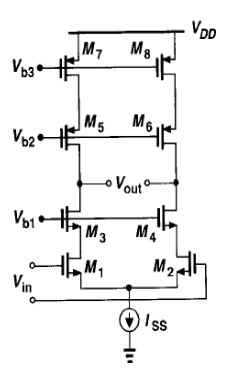
\includegraphics[width=\linewidth]{images/telescopic.png}
\caption{Telescopic OTA}
\label{tele}
\end{minipage}
\hfill
\begin{minipage}[c]{0.5\linewidth}%
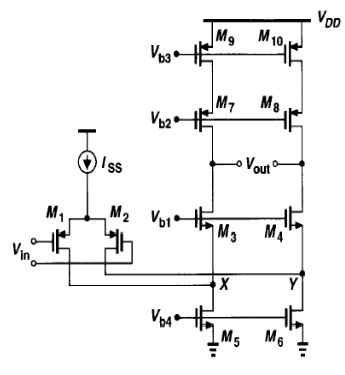
\includegraphics[width=\linewidth]{images/folded.png}
\caption{Folded cascode}
\label{fold}
\end{minipage}%
\end{figure}

\subsection{Single ended vs fully differential output }
In practice, fully differential output is used because it has many advantages over single ended \cite{Johns}. Some being:

\begin{itemize}

\item \textbf{Larger voltage output swing}: since the fully differential has twice as many output as the single ended one, the voltage output swing is almost double in magnitude. 

\item \textbf{Higher SNR}: Since the voltage output swing is large we get a higher signal-to-noise ratio (SNR). The signal output power becomes four times bigger because of twice the output voltage, also the noise power is doubled. Hence we get a overall 3dB improvement in SNR or 0.5 bit improvement in effective number of bits (ENOB).

\item \textbf{Better noise rejection}: It is less susceptibility to common mode noise.
\end{itemize}
One important thing to note with fully differential circuits is that they need additional circuit to keep the output common mode level stable i.e. a common mode feedback circuit is needed, which we will discuss later. This additional circuit causes larger area and higher power consumption compared to single ended topology\cite{Allen}. 

\subsection{The $g_m/I_D$ methodology}

With the emergence of advanced fabric processes the transistor dimensions have reduced drastically. As a consequence the traditional long-channel equations employed in the analog design were no longer producing desired results. In order to treat this inconvenience a new methodology was introduced by F. Silveria, D. Flandre and P. G. A. Jespers \cite{gm_id_1}. The method exploits the relationship between the ratio of the tranceconductance $g_m$ over dc drain current $I_D$ and the normalized drain current $I' = I_D/W$. It uses this relationship to determine the transistor dimensions to satisfy specifications like the GBW, low power, gain, etc. The $g_m/I_D$ ratio can be obtained by characterization of the process of the PMOS and NMOS transistors. Some of the key elements with the $g_m/I_D$  based design are described as follows\cite{gm_id_1},\cite{gm_id_2}:

$\bullet$ This method characterizes the performance of a transistor in all regions of operation. The curve generated for a particular process of a transistor is continuous and there are no transition in equations from various regions of operation, as it would be in the conventional long-channel equations. Thus we can freely select the device operation as per our needs. 

$\bullet$ With the generated curve one can easily derive the transistor dimensions meeting the specifications, as we will see later. 

$\bullet$ The amount of iteration in designing complex analog circuits is drastically reduced. The method gives a complete characterization of the technology, which involving take into account the parasitic influencing the device. Thus eliminating the approximate equation used to determine the device behaviour and improving the time used to design the circuits. 

\subsection{Design procedure of OTA}

The selected folded cascode architecture is illustrated in Fig. \ref{fig:folded_ota_design}, and it shows the currents flowing through the different branches. The input pairs is PMOS differential pair. The flicker noise is less in a PMOS transistor, since its mobility is lower than of NMOS transistor\cite{Johns}. From the slew-rate and load capacitance ($C_L$) values listed in table \ref{spec_ota}, the bias current $I_1$ can be determined:

\begin{equation}\label{I_1}
    I_1 \geq SR*C_L
\end{equation}

As a rule of thumb, the load current $I_2$ should be in the range to keep all the transistors in saturation\cite{Razavi}:

\begin{equation}\label{I_2}
    1.2I_1<I_2<2I_1
\end{equation}

Thus making $I_3$ equal to:

\begin{equation}\label{I_3}
    I_3 = \frac{I_1}{2} + I_2
\end{equation}

\begin{figure}[h]
\centering
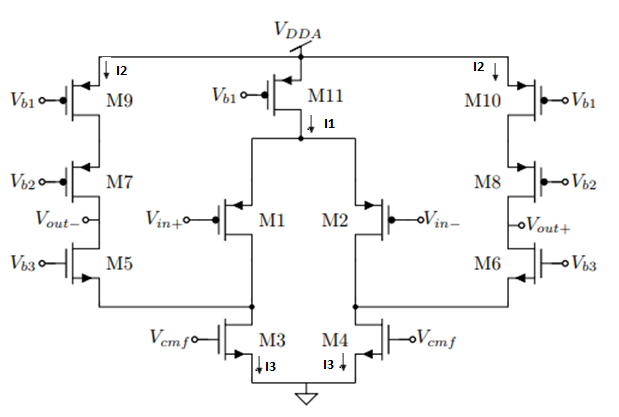
\includegraphics[scale = 0.8]{images/folded_cascode.png}
\caption{Folded cascode architecture with the current $I_1$, $I_2$ and $I_3$ flowing in different branches \cite{Grey}}
\label{fig:folded_ota_design}
\end{figure}

Tranceconductance of the circuit is given by GBW and $C_L$ as follows:

\begin{equation}
    gm_1 = GBW\cdot2\pi\cdot C_L
\end{equation}

The resulting bias currents and the tranceconductance of the circuit of OTA 1, 2 and 3 are listed in \ref{step_1}. These parameters can be used with the $g_m/I_D$ methodology to find the dimensions of the input transistors $M_1$ and $M_2$, as it will be described in the next section. 

\begin{table}[h]
\centering
\caption{The tranceconductance and bias current of OTA 1, 2 and 3}
\label{step_1}
\begin{tabular}{|l|l|l|}
\hline
OTA & $gm_1[\mu S]$ & $I_1[\mu A]$ \\ \hline
1   & 0.85  & 100  \\ \hline
2   & 0.15  & 20   \\ \hline
3   & 0.06   & 10   \\ \hline
\end{tabular}
\end{table}

\subsection{Obtaining transistor dimensions using $g_m/I_D$ methodology}

Using the design flow depicted in Fig.\ref{design_slow}, the procedure to find the dimensions of the transistors can be explained. The $g_m$ and $I_D$ is the tranceconductance and the drain current through a transistor respectively. 

\begin{figure}[H]
\centering
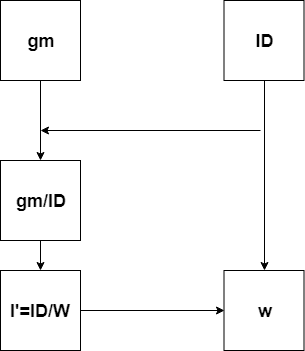
\includegraphics[scale = 0.45]{images/design_flow.png}
\caption{Design flow}
\label{design_slow}
\end{figure}

First step in the device characterization is to generate the plot of $g_m/I_D$ vs $I_D/W$. Fig.
\ref{pmos_setup} shows a PMOS setup in cadence which is used to generate the plot. In a similar manner a NMOS transistor is setup to obtain the same plot. For this simulation transistor dimensions of $\frac{W}{L} = \frac{5\mu}{0.7\mu}$ is chosen. A comparison between the values of PMOS and NMOS transistors is shown in Fig. \ref{fig:comp_pmos_nmos}.

For illustrative purpose we will find the dimensions of transistor $M_1$ of OTA 1 and use the design flow in Fig. \ref{design_slow} to get an insight on how the $g_m/I_D$ method works. From table \ref{step_1} we have that the $gm_1 = 0.85\mu S$ and the drain current through the transistor is given by:

\begin{equation}
    I_{M1} = \frac{I_1}{2} = 50\mu A
\end{equation}

which gives us:

\begin{equation}\label{gm_ID}
   gm_1/I_{M1} = 17 
\end{equation}



\begin{figure}[H]
\centering
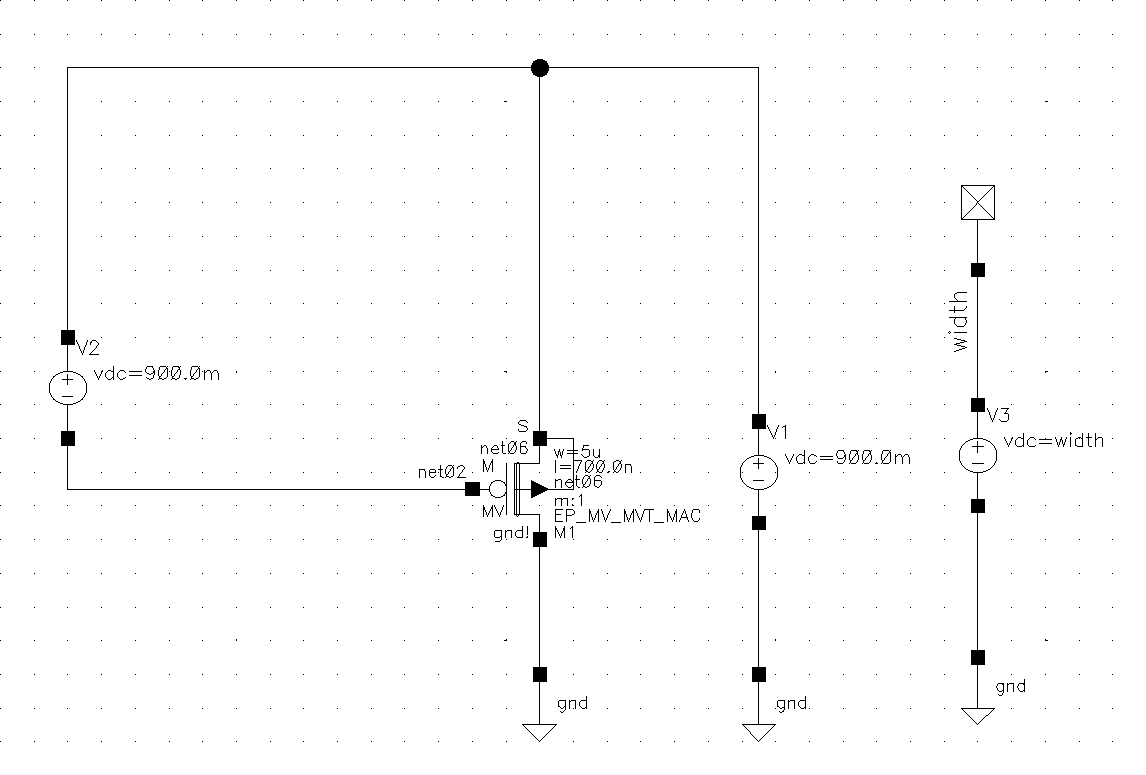
\includegraphics[scale = 0.45]{images/gm_id_pmos_schem.png}
\caption{Schematic of the PMOS transistor setup in cadence}
\label{pmos_setup}
\end{figure}

We then uses $g_m/I_D$ vs $I_D/W$ plot from Fig. \ref{fig:gm_pmos} to obtain the value $I_D/W = 230.137mm$ which corresponds to the $g_m/I_D$ value obtained in equation \ref{gm_ID}. The final width of the transistor is:

\begin{equation}
    W = \frac{I_D}{I_D/W} = 217\mu m
\end{equation}

with the length to the transistor equal to $L = 0.7\mu$, we get:

\begin{equation}
\frac{W}{L} = \frac{217\mu}{0.7\mu} 
\end{equation}


As we will see in the table \ref{final_ota}, this method gives us good accuracy of the desired values needed to satisfy the specifications of the application.


\begin{figure}[ht!]
\centering
\begin{subfigure}[b]{0.85\linewidth}
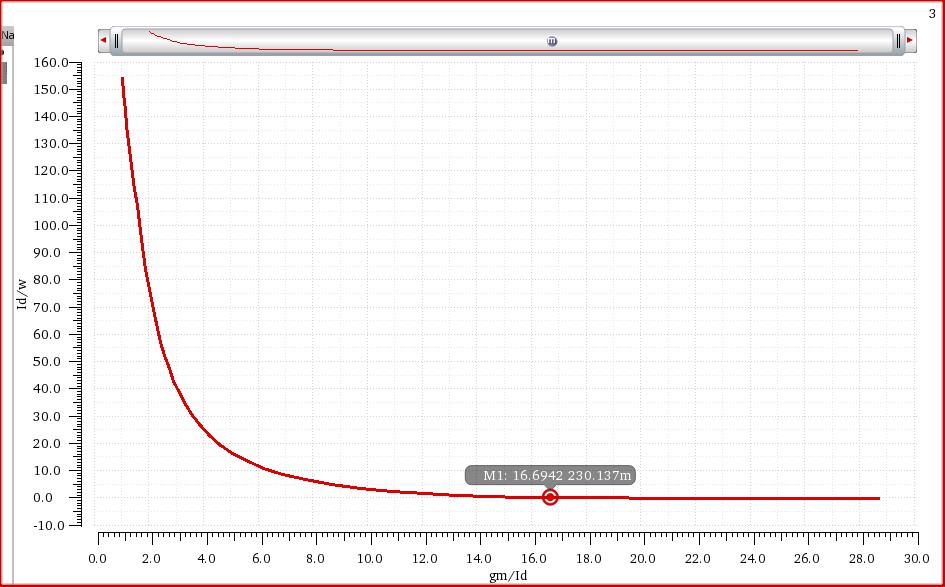
\includegraphics[width = \textwidth]{images/Id_w_vs_gm_id_pmos.jpg}
\caption{PMOS}
\label{fig:gm_pmos}
\end{subfigure}

\begin{subfigure}[b]{0.85\linewidth}
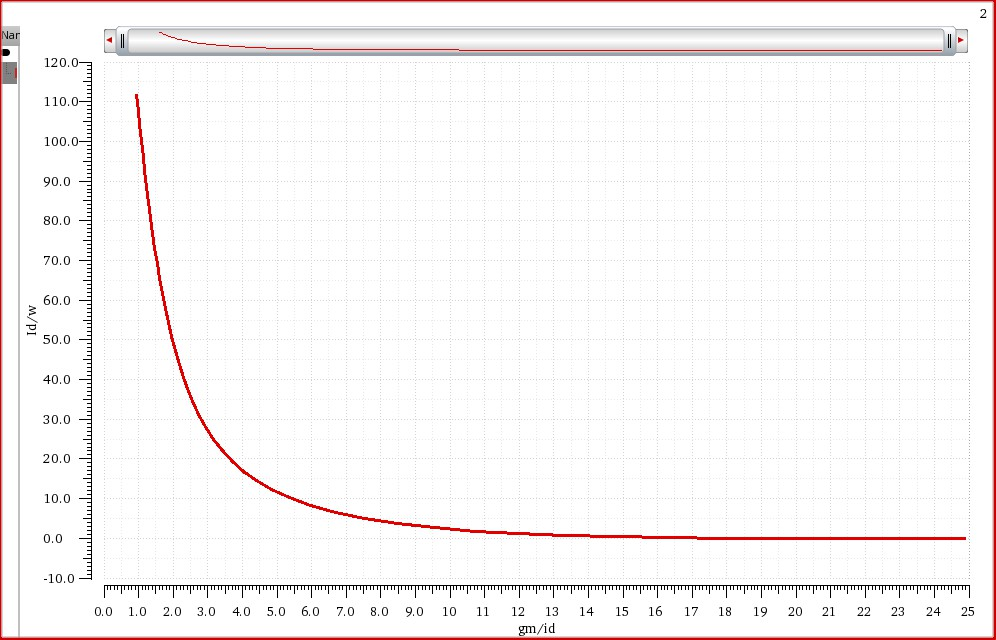
\includegraphics[width = \textwidth]{images/gm_id_w_nmos.jpg}
\caption{NMOS}
\label{fig:gm_nmos}
\end{subfigure}

\caption{Comparison of PMOS and NMOS transistors for $g_m/I_D$ vs $I_D/W$}
\label{fig:comp_pmos_nmos}
\end{figure}


\subsection{Final dimensions of the transistors}

The dimensions for the input transistors of OTA 2 and 3 can be found in a similar manner as it was done for OTA 1 by using table \ref{step_1}, but for transistors $M_3 - M_{11}$ we need to additionally  look at the output-swing specification given i table \ref{spec_ota} for the different OTAs. For folded cascode we have a maximum output voltage swing requirement given by\cite{Razavi}:

\begin{equation}
    VO_{max} = V_{DDA} - (V_{OD7} + V_{OD9})
\end{equation}

\begin{equation}
    VO_{min} = V_{OD3} + V_{OD5}
\end{equation}

Where $VO_{max}$ is the upper end and $VO_{min}$ is the lower end of the swing. $V_{OD}$ is the overdrive voltage which define the region the transistor operate in, and is given by the gate voltage and threshold voltage of the transistor:

\begin{equation}
    V_{OD} = V_{GS} - V_{th}
\end{equation}

Since $V_{GS}$ depends on the bias voltage $V_{b}$ we can freely choose which region a transistor will operate in. Transistors in strong inversion has poor current efficiency and low output range, but it is small and the transient frequency is high. Transistors in weak inversion on the other hand has good current efficiency and high output voltage range, but at the cost of a larger transistor and low transient frequency. Moderate inversion is a good compromise between these two regions \cite{gm_id_2}. The goal was to size the transistor to operate as close as possible in this region, thus having good output voltage range while maintaining small area. 

The next step is to use $g_m/I_D$ method to find dimensions for the transistors. The drain current through each transistor can be find using equations: \ref{I_1}, \ref{I_2} and \ref{I_3}. The tranceconductance ($g_m$) of the transistors can be expressed with the help of $V_{OD}$ as follows:

\begin{equation}
    gm = \sqrt{2I_DC_{ox}\frac{W}{L}} = \frac{2I_D}{V_{OD}}
\end{equation}

With the right choice of $V_{OD}$ we can compute the $g_m/I_D$ for a transistor that operate in the moderate inversion region. Then we can use the value of $g_m/I_D$ with the plot in Fig. \ref{fig:gm_pmos} or \ref{fig:gm_nmos} (depending on if we look at PMOS or NMOS transistor) to find the dimension of the transistor, as it was done for transistor $M_1$. This procedure was used as a starting point for sizing the transistors. The final dimensions for the three OTAs were set by using PVT simulations and are summarized in table \ref{final_ota}. The design accomplished the requirements mentioned in table \ref{spec_ota}, as it will be seen in chapter \ref{res:results}.

\begin{table}[h]
\centering
\caption{Transistor dimensions of OTA 1, 2 and 3}
\label{final_ota}
\begin{tabular}{l||l|l||l|l||l|l}
\hline
\multirow{2}{*}{Device} & \multicolumn{2}{c||}{$OTA_1$} & \multicolumn{2}{c||}{$OTA_2$} & \multicolumn{2}{c}{$OTA_3$}\\\cline{2-7}
                        &W[$\mu m$] & L[$\mu m$]& W[$\mu m$] & L[$\mu m$] & W[$\mu m$] & L[$\mu m$]\\\hline
            $M_1$       & 217 & 0.7 & 180 & 0.7 & 163 & 0.7\\
            $M_2$        & 217 & 0.7 & 180 & 0.7 & 163 & 0.7\\
            $M_3$        & 126 & 1 & 97 & 1 & 81 & 1\\
            $M_4$        & 126 & 1 & 97 & 1 & 81 & 1\\
            $M_5$        & 23 & 0.7 & 35 & 0.7 & 25 & 0.7\\
            $M_6$        & 23 & 0.7 & 35 & 0.7 & 25 & 0.7\\
            $M_7$        & 87 & 0.7 & 70 & 0.7 & 52 & 0.7\\
            $M_8$        & 87 & 0.7 & 70 & 0.7 & 52 & 0.7\\
            $M_9$        & 56 & 1 & 43 & 1 & 40 & 1\\
            $M_{10}$        & 56 & 1 & 43 & 1 & 40 & 1\\
            $M_{11}$        & 98 & 1 & 77 & 1 & 66 & 1\\
\hline            
\end{tabular}
\end{table}

\subsection{Bias circuit}

\begin{figure}[h!]
\centering
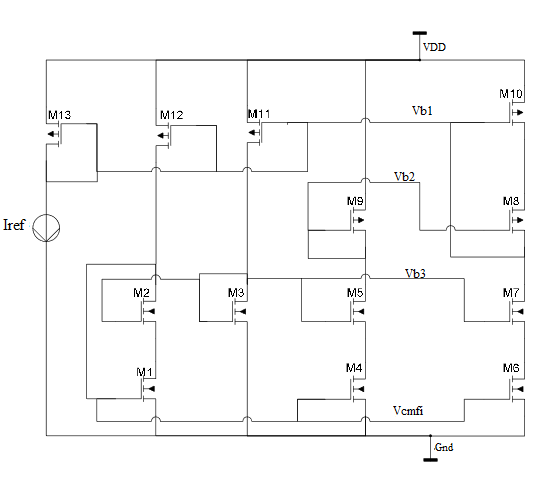
\includegraphics[scale = 0.7]{images/bias_circuit.png}
\caption{Wide swing current mirror}
\label{bias circuit}
\end{figure}

The points $V_{b1}$, $V_{b2}$ and $V_{b3}$ in Fig. \ref{fig:folded_ota_design} are the DC voltages used to bias the transistors, while $V_{cmf}$ controls the common output mode of the OTA. Figure \ref{bias circuit} shows a wide swing current mirror \cite{Allen} which is used to generate the necessary bias voltages in the cascode pair. A wide swing current mirror topology has the perks of not limiting the signal swing as much as the other conventional current mirrors. It also provides a better matching of the currents and higher output resistance. To get a lower power consumption the reference current $I_{ref}$ is set to $10\mu A$, $2\mu A$ and $1\mu A$ for OTA 1, 2 and 3 respectively. With such low currents, especially for OTA 2 and 3, large amounts of noise are generated. This will not be a problem for our ADC, since the noise will be considerably attenuated for OTA 2 and 3. The transistors $M_1-M_3$ and $M_{11}-M_{13}$ are made ten times smaller than the transistors in the cascode of the OTAs. While the dimensions of the transistors $M_{4} - M_{10}$ are the same as the one used in the cascode to make sure that the bias currents listed in table \ref{step_1} are properly mirrored into the OTAs. Transistors $M_3$ and $M_9$ are made four times smaller than transistors $M_2$ and $M_8$ respectively to ensure proper generation of the bias voltages\cite{Johns}. The gate length of the transistors are made to be approximately two times longer than the allowable minimum length to get better matching during layout. Table \ref{final_bias} summarize the transistors dimensions of the circuit for OTA 1, 2 and 3.    

\begin{table}[]
\centering
\caption{Transistor dimensions of the OTAs bias circuits}
\label{final_bias}
\begin{tabular}{l||l|l||l|l||l|l}
\hline
\multirow{2}{*}{Transistor} & \multicolumn{2}{c||}{$OTA_1$} & \multicolumn{2}{c||}{$OTA_2$} & \multicolumn{2}{c}{$OTA_3$}\\\cline{2-7}
                        &W[$\mu m$] & L[$\mu m$]& W[$\mu m$] & L[$\mu m$] & W[$\mu m$] & L[$\mu m$]\\\hline
            $M_1$       & 12.6 & 1 & 9.7 & 1 & 8.1 & 1\\
            $M_2$        & 3.3 & 1 & 5.6 & 1 & 3.6 & 1\\
            $M_3$        & 0.82 & 1 & 1.4 & 1 & 0.9 & 1\\
            $M_4$        & 126 & 1 & 97 & 1 & 81 & 1\\
            $M_5$        & 32.8 & 1 & 56 & 1 & 35.7 & 1\\
            $M_6$        & 126 & 1 & 97 & 1 & 81& 1\\
            $M_7$        & 32.8 & 1 & 56 & 1 & 35.7 & 1\\
            $M_8$        & 124.3 & 1 & 100 & 1 & 74.3 & 1\\
            $M_9$        & 31.1 & 1 & 25 & 1 & 18.6 & 1\\
            $M_{10}$        & 98 & 1 & 77 & 1 & 66 & 1\\
            $M_{11}$        & 9.8 & 1 & 7.7 & 1 & 6.6 & 1\\
            $M_{12}$        & 9.8 & 1 & 7.7 & 1 & 6.6 & 1\\
            $M_{13}$        & 9.8 & 1 & 7.7 & 1 & 6.6 & 1\\
\hline            
\end{tabular}
\end{table}
\clearpage

\subsection{Common mode feedback block}
As mentioned one of the biggest disadvantage of a fully differential OTAs is that; if the common mode output is not controlled it can either go to positive or negative rail and thereby drive some transistors out of the saturation/active region. Hence an additional circuit is required to keep the common mode output stable. Figure \ref{cmfb} shows a switched capacitor common mode feedback block which is a simple circuit used generally in discrete-time circuit. The circuit produce the output common mode voltage by comparing the average of the differential output voltages with the desired common mode voltage. Then the difference between these two voltage ($V_{cmf}$) is used to bring the OTA's common mode voltage back to the desired common mode level. Since the stability of the OTA gets changed when introducing extra capacitors at the output, capacitor $C_1$ and $C_2$ has to be chosen with care. The values were determined by simulation, as a rule of thumb capacitor $C_2$ should be five times larger than $C_1$\cite{Johns}. Table \ref{final_cmfb} list up the capacitance values for OTA 1, 2 and 3. 
\begin{figure}[h!]
\centering
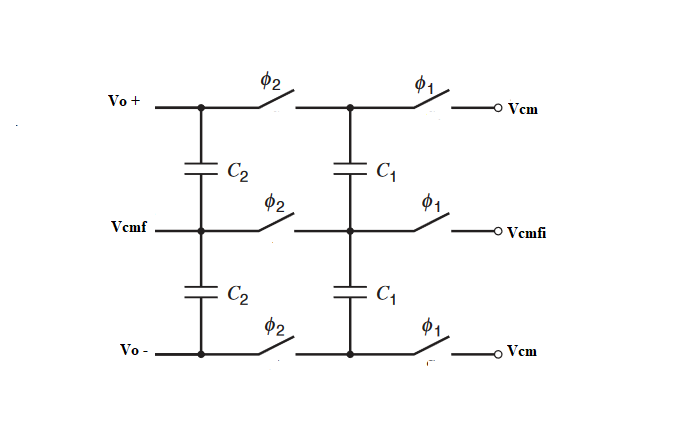
\includegraphics[scale = 0.7]{images/cmf_circuit.png}
\caption{Switched capacitor CMFB circuit\cite{Grey}}
\label{cmfb}
\end{figure}

\begin{table}[h!]
\centering
\caption{CMFB capacitance values}
\label{final_cmfb}
\begin{tabular}{l|l|l|l}
\hline
\multirow{1}{*}{Capacitor} & \multicolumn{1}{c|}{$OTA_1$} & \multicolumn{1}{c|}{$OTA_2$} & \multicolumn{1}{c}{$OTA_3$}\\\cline{1-4}
                       
            $C_1[pF]$       & 1 & 1.35 & 2.1\\
            $C_2 [pF]$      & 0.2 & 0.27 & 0.42 \\
            
\hline            
\end{tabular}
\end{table}

\section{Quantizer}

The quantizer in a $\Delta\Sigma$ ADC has to work at a high oversampling frequency, but its resolution is 1-bit. Therefore we have chosen to implement a latched comparator\cite{comparator} shown in Fig. \ref{quantizer} that focus more on high-speed operation than accuracy. The comparator is clocked in order to synchronize its operation with other circuits in the ADC. The main parameter of concern was  hysteresis, since the input offset and input referred noise get attenuated by the feedback loop of the modulator. 

\begin{figure}[h]
\centering
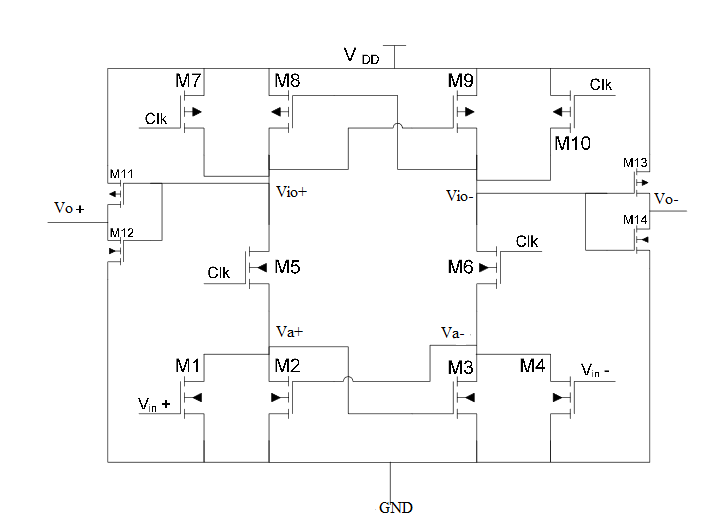
\includegraphics[scale = 0.7]{images/quatizier_circuit.png}
\caption{Latched comparator\cite{comparator}}
\label{quantizer}
\end{figure}

The input $M_1$ and $M_4$ are the discharge controlling transistors which are connected to the flip-flop $M_2$ and $M_3$ in a feedback network. $M_5$ and $M_6$ are control transistors which keep track of holding the comparator synchronized with the rest of the ADC. $M_8$ and $M_9$ are another flip-flop connected in feedback with transistors $M_7$ and $M_{10}$, which are precharge transistors used for refreshing the internal nodes when they are not in operation, to reduce hysteresis. Inverters $M_{11-12}$ and $M_{13-14}$ act as buffers to isolate the latch from the output load and to amplify the comparator output.

When the \textit{Clk} is low, transistors $M_5$ and $M_6$ gets cut off and the input signal will not influence the comparator. The voltages $V_{io+}$ and $V_{io-}$ will be pulled to the positive rail $V_{DD}$, and because of the inverters the output will be pulled to ground. At the same time the voltages $V_a+$ and $V_a-$ gets discharged to ground by transistors $M_1$ and $M_4$. Suppose $V_{in+}$ is greater than $V_{in-}$. When the \textit{Clk} goes high, both voltages $V_{io+}$ and $V_{io-}$ drop from the positive rail and the voltages $V_a+$ and $V_a-$ rise from the ground. However, $M_1$ draws more current than $M_2$, and thereby more current is flowing through $M_3$. This causes $V_{a-}$ to rise faster than $V_{a+}$. Since more current flows through $M_5$ than $M_6$, the voltage $V_{io+}$ drops faster than $V_{io-}$. The regenerative action of $M_8$ and $M_9$ together with that of $M_2$ and $M_3$ pulls $V_{io+}$ to ground and pulls $V_{io-}$ to positive rail. Hence, $V_{0+}$ goes high while $V_{0-}$ goes low. The operation is similar when $V_{in-}$ is greater than $V_{in+}$.

The circuit has digital behaviour with the exception of transistors $M_1$ and $M_4$ that amplify the input signal. Hence, the transistors that operate as digital circuit have minimum dimensions, while the input transistors have a larger length to avoid mismatch effects. The transistor dimensions are listed up in table \ref{final_comparator}.

\begin{table}[]
\centering
\caption{Transistor dimensions of the latched comparator}
\label{final_comparator}
\begin{tabular}{l|l|l}
\hline
\multirow{1}{*}{Transistor} & \multicolumn{1}{c|}{W[$\mu m$]} & \multicolumn{1}{c}{L[$\mu m$]} \\\cline{1-3}
                       
            $M_1$       & 1 & 1\\
            $M_2$      & 0.5 & 0.55\\
            $M_3$      & 0.5 & 0.55\\
            $M_4$      & 1 & 1\\
            $M_5$      & 0.5 & 0.55\\
            $M_6$      & 0.5 & 0.55\\
            $M_7$      & 1 & 0.55\\
            $M_8$      & 1 & 0.55\\
            $M_9$      & 1 & 0.55\\
            $M_{10}$      & 1 & 0.55\\
            $M_{11}$      & 0.5 & 0.55\\
            $M_{12}$      & 0.5 & 0.55\\
            $M_{13}$      & 0.5 & 0.55\\
            $M_{14}$      & 0.5 & 0.55\\
            
\hline            
\end{tabular}
\end{table}

Finally, the output of the comparator is only valid in phase $\phi_1$, and the output of the feedback DAC gets sampled on integrator 1 at phase $\phi_2$. In order to keep the comparator output valid in both phases, a SR-latch is placed in front of the comparator. Since the circuit is purely digital, the dimensions are also here set to minimum. The SR-latch is shown in Fig. \ref{app:SR} in appendix \ref{app:cicuits}.

\section{Non-overlapping clock generator}
The implemented clock generator is a two-phase non-overlapping circuit. It was designed with the intention of maximize the time available, and make the early and late phases start at the same time, i.e. $\phi_1$ and $\phi_{1d}$ start at the same time. The same apply for phases $\phi_2$ and $\phi_{2d}$. The generator consists of NAND-gates and inverters as shown in Fig. The logic gates have minimum dimensions where the dimensions of the PMOS transistors is three times the NMOS ones. Further delayed clock can be produced by adding more delay inverters on the path from the outputs of the generator to the input of the NOR-gates. Since the switches are transmission gates, each phase needs a complementary singal for proper operation. Complementary signals $\overline{\phi_1}$, $\overline{\phi_{1d}}$, $\overline{\phi_2}$ and $\overline{\phi_{2d}}$ are realized by putting an inverter in front of the outputs of the generator. 

\begin{figure}[h]
\centering
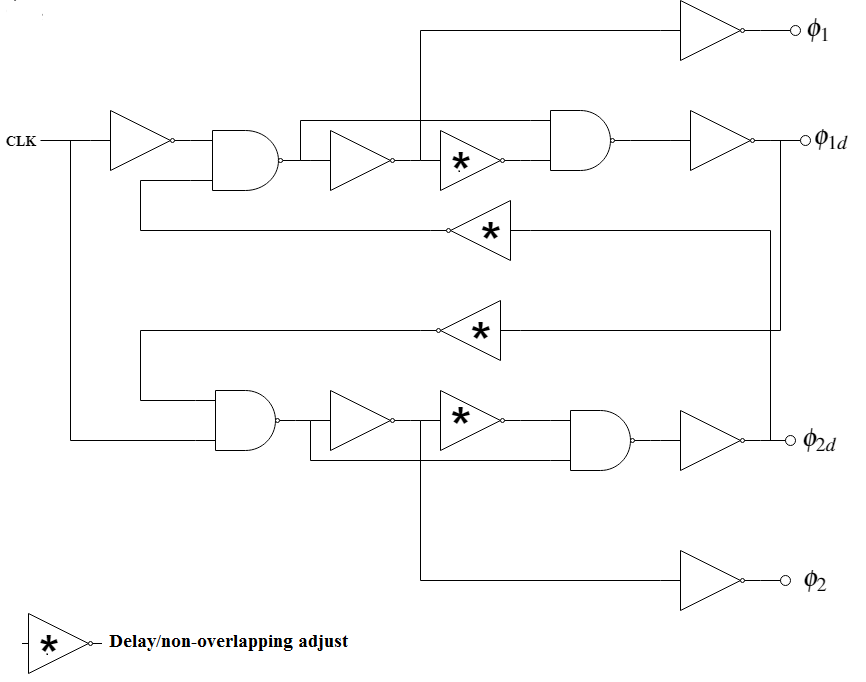
\includegraphics[scale = 0.5]{images/two_phase_clock.png}
\caption{1-bit DAC}
\label{clock_block}
\end{figure}


\section{DAC}
The 1-bit DAC implemented is shown in Fig. \ref{DAC_block}, and the functionality is simple. For instance, depending on if the input signal dacp\_1 is either high or low the feedback out back to integrator 1 is either vrefp or vrefn which is the reference voltages. Similarly the output vfbp depends on the level of input dacn\_1. In a differential circuit, the reference voltages must be centered at the analog ground $V_{cm} = 0.9V$. Hence, they have to be implemented so they are symmetric with respect to $V_{cm}$ such that their difference is equal to $V_{ref}$ (listed in table \ref{spec}). The reference voltages are chosen to be $\pm 0.5$ around $V_{cm}$. Therefore, vrefp is 1.4V and vrefn is 0.4V. The switches is implemented as TG switch with the dimensions of PMOS switch being $\frac{W}{L}_p = \frac{10.5}{0.55}\mu m$ and $\frac{W}{L}_n = \frac{3.5}{0.55}\mu m$, giving an on-resistance of $905.4\Omega$. 

\begin{figure}[]
\centering
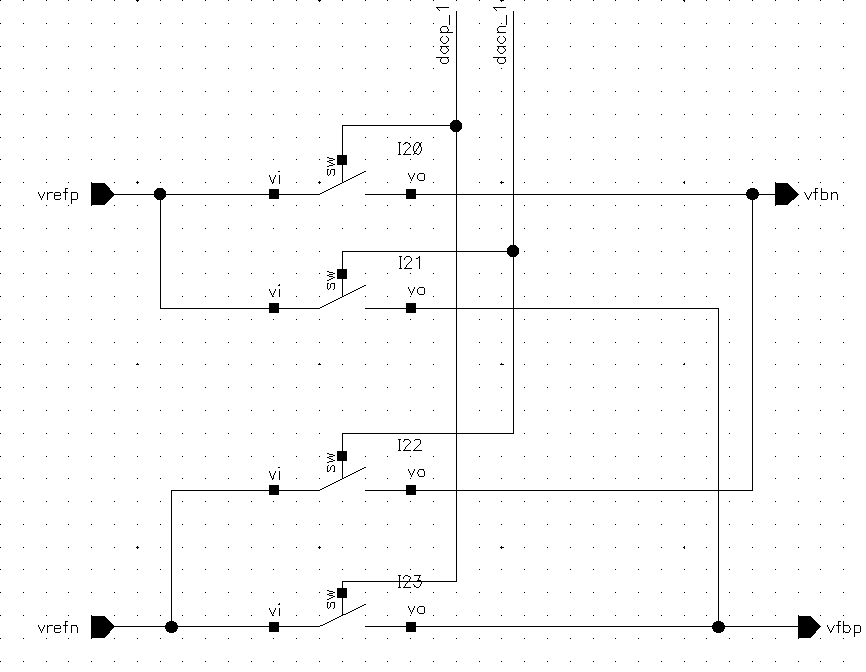
\includegraphics[scale = 0.45]{images/DAC_block.png}
\caption{1-bit DAC}
\label{DAC_block}
\end{figure}
\chapter{Results}\label{res:results}

The results for the analog blocks were obtained by using spectre simulator in Cadence Virtuoso ADE. In case of noise simulation a transient noise was imposed. The functionality and integrity of the modulator and the analog blocks were validated using Nominal simulation. Additionally PVT simulations were performed on the modulator,the OTAs,the quantizer and the clock generator in order to verify the robustness of these blocks. The nominal simulation operate with typical transistor model at room temperature and standard supply voltage. PVT simulation on the other hand operate with corner models of the the process where the range of the temperatures are between $-40^\circ$ and $105^\circ$, and 2.5 V and 5.5 V for the supply voltage. Furthermore it also consists of performing many simulations based on the statistical model of the transistors, namely 16. The corners model of the transistors provided by Microchip Technology are: slow, fast, slow-NMOS-fast-PMOS (SNFP) and fast-NMOS-slow-PMOS (FNSP). 


\section{Non-overlapping clock}
The output signals from the designed non-overlapping clock generator is shown in Fig. \ref{clock_out}. The non-overlapping time is 23.52nsec between $\phi_1$ and $\phi_2$, and $\phi_{1d}$ is delayed from $\phi_1$ with 10nec, the same delay apply for $\phi_{2d}$ and $\phi_2$. It should be noted that the delays are not affected by mismatch effects and process variation. 

\begin{figure}[h]
\centering
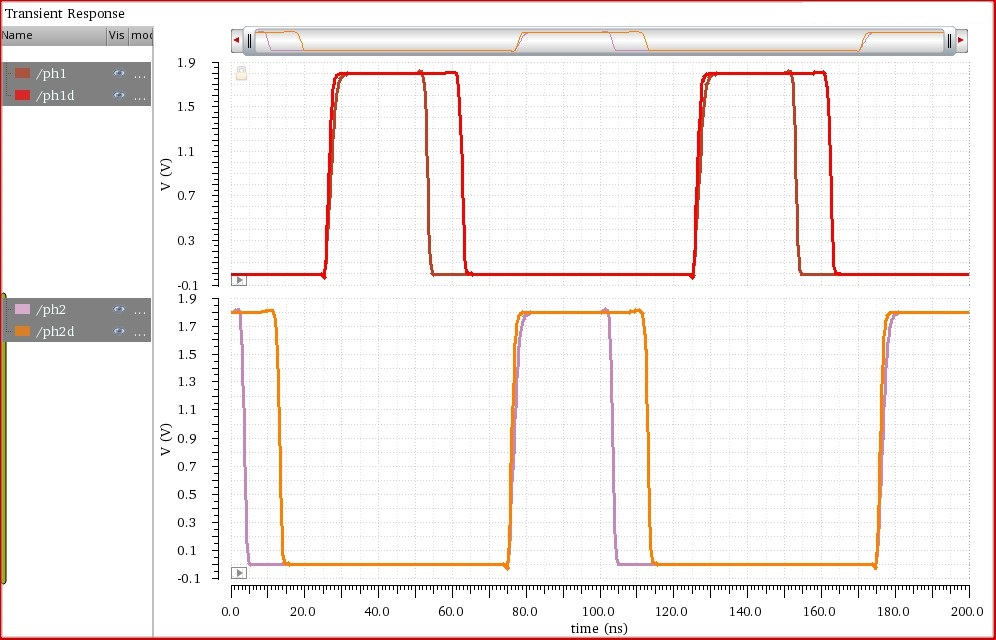
\includegraphics[width=\textwidth]{images/two_phase_clock_out.jpg}
\caption{Clock phases}
\label{clock_out}
\end{figure}

\section{Quantizer}
The quantizer used is simply a latched comparator which switches to the rail supply depending on the input signals. It is designed as per the methodology discussed earlier. The quantizer was simulated using three input signals: $V_{in+}$, $V_{in-}$ and CLK. The positive and negative input voltages are signals that vary from ground to $V_{DD}$ and from $V_{DD}$ to ground respectively. The output only changes at the rising edge of the clock. As mentioned in the methodology the hysteresis parameter was used to validate the quantizer, since the input offset and the input referred noise get attenuated by the feedback loop of the modulator. Figure \ref{comparator_out} shows when the output gets updated as the input voltages $V_{in+}$ and $V_{in-}$ vary. Due to the regenerative latch the hysteresis of the quantizer was measured as small as 5.86$m V/V$. PVT simulations were performed with no corners being critical to the quantizer's performance. 

\begin{figure}[H]
\centering
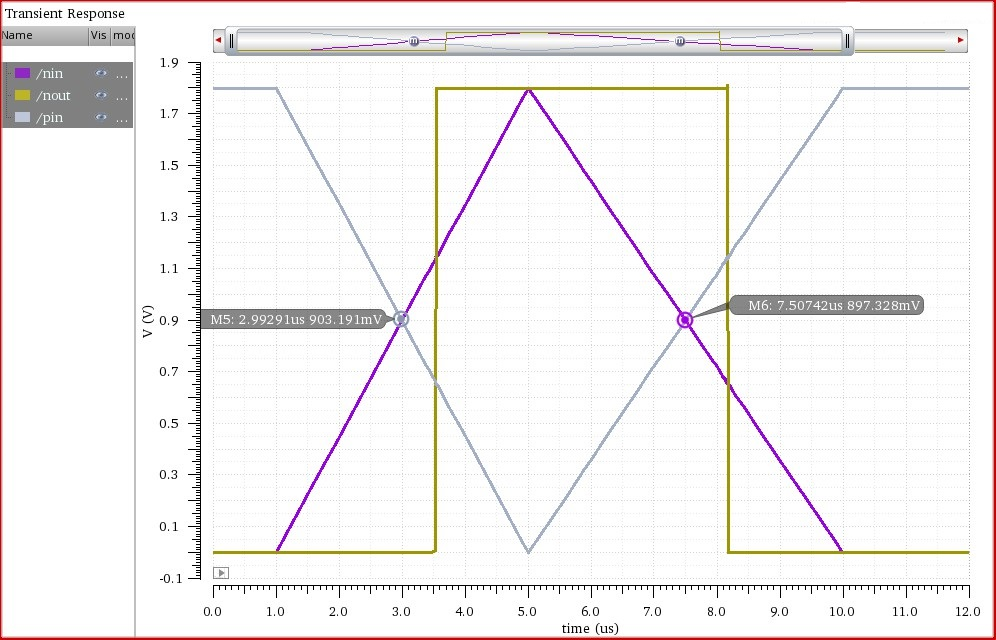
\includegraphics[width=\textwidth]{images/Comperator_output.jpg}
\caption{Hysteresis of the comparator}
\label{comparator_out}
\end{figure}


\section{OTA}
With the use of nominal and PVT simulation the specifications were validated. The results of the simulation are based on the set of requirements listed in table \ref{spec_ota}. 

\subsection{Nominal simulations}

\begin{table}[h]
\centering
\caption{Nominal results from OTA 1, 2 and 3}
\label{nominal_ota}
\begin{tabular}{l|l|l|l}
\hline
\multirow{1}{*}{Specification} & \multicolumn{1}{c|}{OTA 1} & \multicolumn{1}{c|}{OTA 2} & \multicolumn{1}{c}{OTA 3}  \\\cline{1-4}
                       
            DC gain       & 60dB & 42dB & 40dB\\
            GBW      & 43.2MHz & 36.7MHz & 38.2MHz\\
            Phase margin     & 75.6$^\circ$ & 70$^\circ$ & 78.4$^\circ$\\
            Power    & 22.3$\mu$W & 11.7$\mu$W & 8.5$\mu$W\\
            Slew rate   & 42.12MV/sec & 46.23MV/sec & 47.76MV/sec\\
            Maximum output voltage    & 1.15 & 1.2 & 1\\
            Minimum output voltage     & 0.65 & 0.65 & 0.7\\
            
\hline            
\end{tabular}
\end{table}

The main results of the nominal simulations of OTA 1, 2 and 3 are listed in table \ref{nominal_ota}, and frequency responses are depicted in Fig. \ref{frequrncy_out}. As discussed in chapter 3 the specifications of the OTAs are indeed relaxed, which made the design process that much easier. The DC-gain and GBW fulfill the specifications with good margin for all three OTAs. Even with the common mode feedback block which effect the stability, the phase margin of the three OTAs exceeds the requirements. Additionally the power consumption including the bias circuit were around 22.3 $\mu W$, 11.7$\mu W$ and 8.5$\mu W$ for OTA 1, 2 and 3 respectively. One thing to notice is that the power consumption of OTA 1 is greater than for OTA 2 and 3 due to the slew rate requirement. Different topologies can be used to reduce the power consumption of OTA 1, such as an adaptive bias circuit \cite{adaptive}. It has the advantage of improving the power efficiency while achieving high slew rate. 

\begin{figure}[H]
\centering
\begin{subfigure}[b]{0.85\textwidth}
   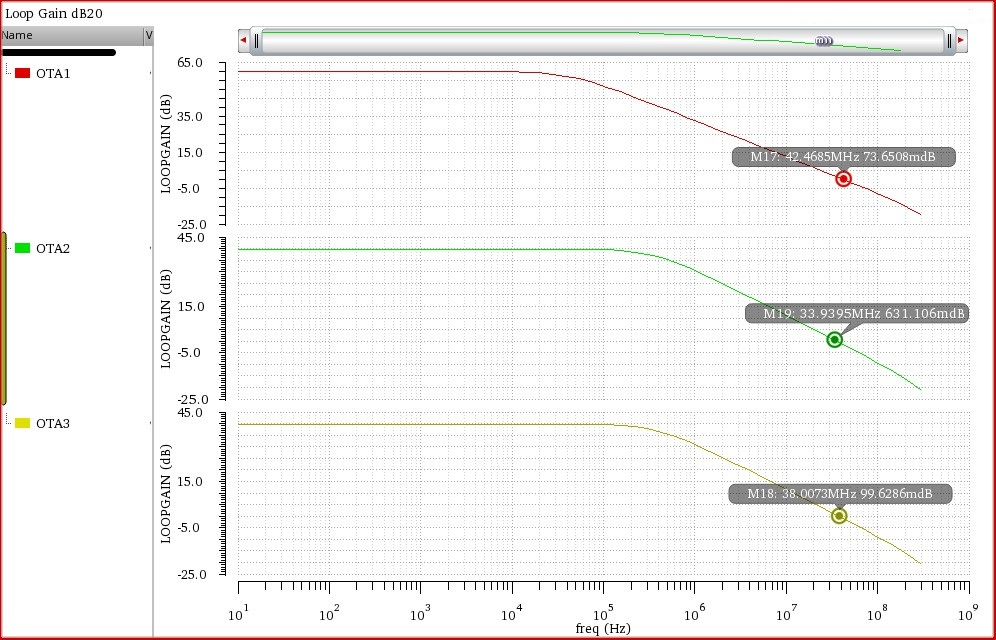
\includegraphics[width=\textwidth]{images/nom_GBW_1_2_3.jpg}
\end{subfigure}

\begin{subfigure}[b]{0.85\textwidth}
   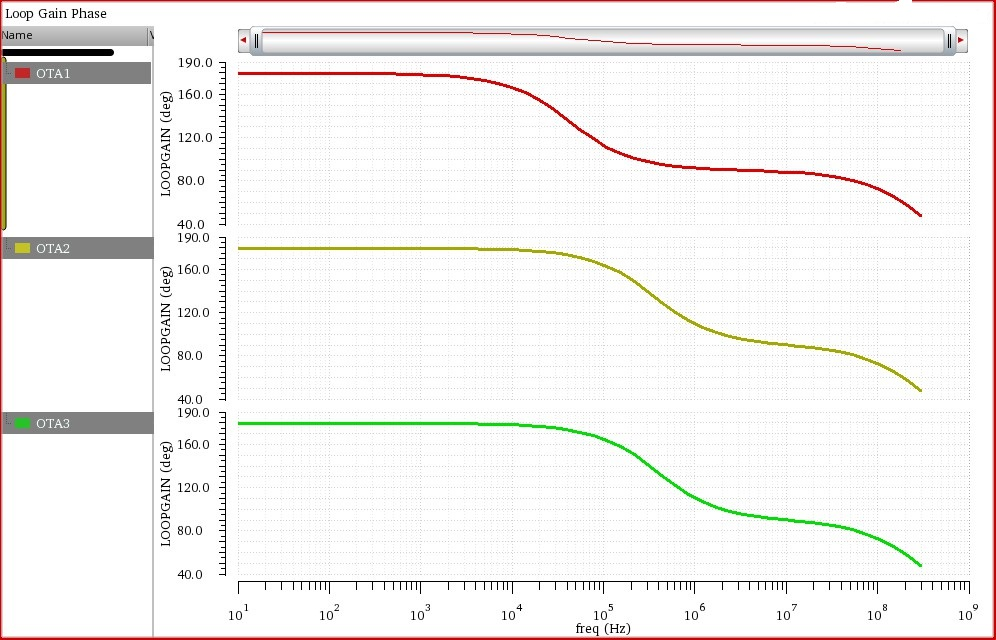
\includegraphics[width=\textwidth]{images/nom_phase_1_2_3.jpg}
\end{subfigure}

\caption{Frequency response of OTA 1,2 and 3}
\label{frequrncy_out}
\end{figure}

The maximum and minimum output voltages of OTA 1 and 2 are within the requirements in table \ref{spec_ota} with headroom to spare, since the transistors $M_3$, $M_4$, $M_9$ and $M_10$ operated in moderate region. However the maximum and minimum output voltages of OTA 3 fulfill the requirements just barley. This will not affect the performance of the modulator as it will be seen in subsequent sections. 
\begin{figure}[H]
\centering
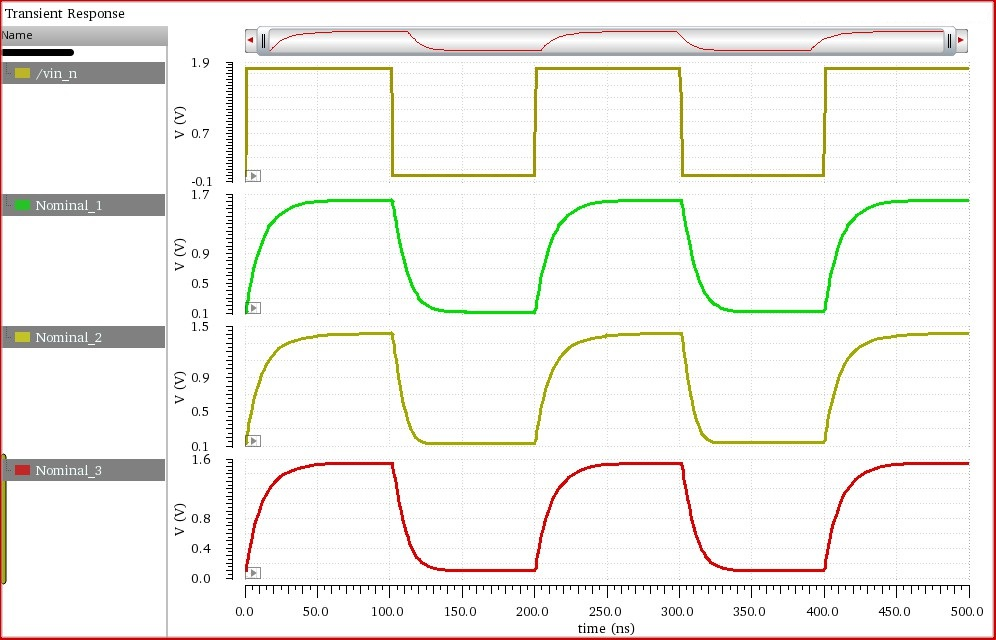
\includegraphics[width=\textwidth]{images/nominal_slew_rate_1_2_3.jpg}
\caption{Slew rate of OTA 1, 2 and 3 }
\label{slew_rate_out}
\end{figure}

The slew rates of the OTAs were found to be 42.12MV/sec, 46.23MV/sec 47.76MV/sec for OTA 1, 2 and 3 respectively, shown in Fig \ref{slew_rate_out}. With these high slew rates one can ensure that the non-linear settling error will not occur. 



\subsection{PVT simulations}
Table \ref{pvt_ota} summarize the maximum and minimum values of the OTAs 1, 2 and 3 parameters for the PVT simulations. It can be seen that the results fulfill the specifications of the amplifier. Table \ref{corners} list up the different environment used to perform the PVT simulations.


\begin{table}[H]
\centering
\caption{PVT results for OTA 1, 2 and 3}
\label{pvt_ota}
\begin{tabular}{l|l|l|l|l}
\hline
\multirow{2}{*}{Specification} & \multicolumn{2}{c|}{Minimum} & \multicolumn{2}{c}{Maximum} \\\cline{2-5}
            & Corner & Value & Corner & Value  \\\hline
            DC gain 1 &Corner 10 & 58.6dB & Corner 11 & 63.4dB \\
            DC gain 2 & Corner 6 & 39.2dB & Corner 11 & 43.3dB \\
            DC gain 3 & Corner 10 & 38.7dB & Corner 11 & 41.8dB \\\hline
            GBW 1    & Corner 3 & 40.63MHz & Corner 6 & 47.13MHz \\
            GBW 2    & Corner 3 & 33.7MHz & Corner 6 & 40.3MHz \\
            GBW 3    & Corner 3 & 34.1MHz & Corner 6 & 41.5MHz \\\hline
            Phase margin 1  & Corner 6 & 70.5$^\circ$ & Corner 13 & 81.4$^\circ$ \\
            Phase margin 2  & Corner 6 & 67.1$^\circ$ & Corner 15 & 75.5$^\circ$ \\
            Phase margin 3  & Corner 6 & 71.4$^\circ$ & Corner 15 & 82.8$^\circ$ \\\hline
            Power 1  & Corner 0 & 14.5$\mu$W & Corner 3 & 45.3$\mu$W \\
            Power 2  & Corner 0 & 7.6$\mu$W & Corner 3 & 22.5$\mu$W \\
            Power 3  & Corner 0 & 4.7$\mu$W & Corner 3 & 17.3$\mu$W \\\hline
            Slew rate 1  & Corner 5 & 36.9MV/sec & Corner 10 & 48.31MV/sec \\
            Slew rate 2  & Corner 5 & 40.3MV/sec & Corner 6 & 50.4MV/sec \\
            Slew rate 3  & Corner 5 & 38.9MV/sec & Corner 6 & 51.2MV/sec \\
            
\hline            
\end{tabular}
\end{table}

The most critical environment for all three OTAs is corner 3, where the power consumption is the largest and the GBW is the lowest. However the GBW still satisfy the requirement for the minimum allowed value for all three OTAs to assure a stable charge transfer.

\begin{table}[H]
\centering
\caption{PVT Corners}
\label{corners}
\begin{tabular}{l|l|l|l}
\hline
\multirow{1}{*}{Corners} & \multicolumn{1}{c|}{Transistor model} & \multicolumn{1}{c|}{Supply voltage} & \multicolumn{1}{c}{Temperature} \\\cline{1-4}
                       
            Corner 0       & slow & 2.5 V & -40$^\circ$\\
            Corner 1      & slow & 2.5 V & 105$^\circ$\\
            Corner 2      & slow & 5.5 V & -40$^\circ$\\
            Corner 3      & slow & 5.5V & 105$^\circ$\\
            Corner 4      & fast & 2.5 V & -40$^\circ$ V\\
            Corner 5      & fast & 2.5 V & 105$^\circ$\\
            Corner 6      & fast & 5.5 V &-40$^\circ$\\
            Corner 7      & fast & 5.5 V & 105$^\circ$\\
            Corner 8      & SNFP & 2.5 V & -40$^\circ$V\\
            Corner 9      & SNFP & 2.5 V & 105$^\circ$\\
            Corner 10      & SNFP & 5.5 V & -40$^\circ$\\
            Corner 11      & SNFP & 5.5 V & 105$^\circ$\\
            Corner 12      & FNSP & 2.5 V& -40$^\circ$\\
            Corner 13      & FNSP & 2.5 V & 105$^\circ$\\
            Corner 14      & FNSP & 5.5 V & -40$^\circ$\\
            Corner 15      & FNSP & 5.5 V & 105$^\circ$\\
            
\hline            
\end{tabular}
\end{table}

Power consumption is nearly double of the nominal value for all three OTAs in corner 3, with the consumption of OTA 1 being noticeable big i.e. 45.4 $\mu W$. The technique mentioned in the previous section can be used to reduce it.   

Figures \ref{corner_freq_1}, \ref{corner_freq_2} and \ref{corner_freq_3} illustrate the plots of the frequency responses for all corners for OTA 1, 2 and 3 respectively. As seen the DC gain for OTA 1 and 3 are worst in corner 10, while for OTA 2 it is worst in corner 6. Both corners have high supply voltage and low temperature. Nevertheless the DC gains satisfy the specifications of table \ref{spec_ota} with good margin. The phase margins also fulfill the specifications in the worst corner 6, and thereby ensuring fastest settling time.  

\begin{figure}[H]
\centering
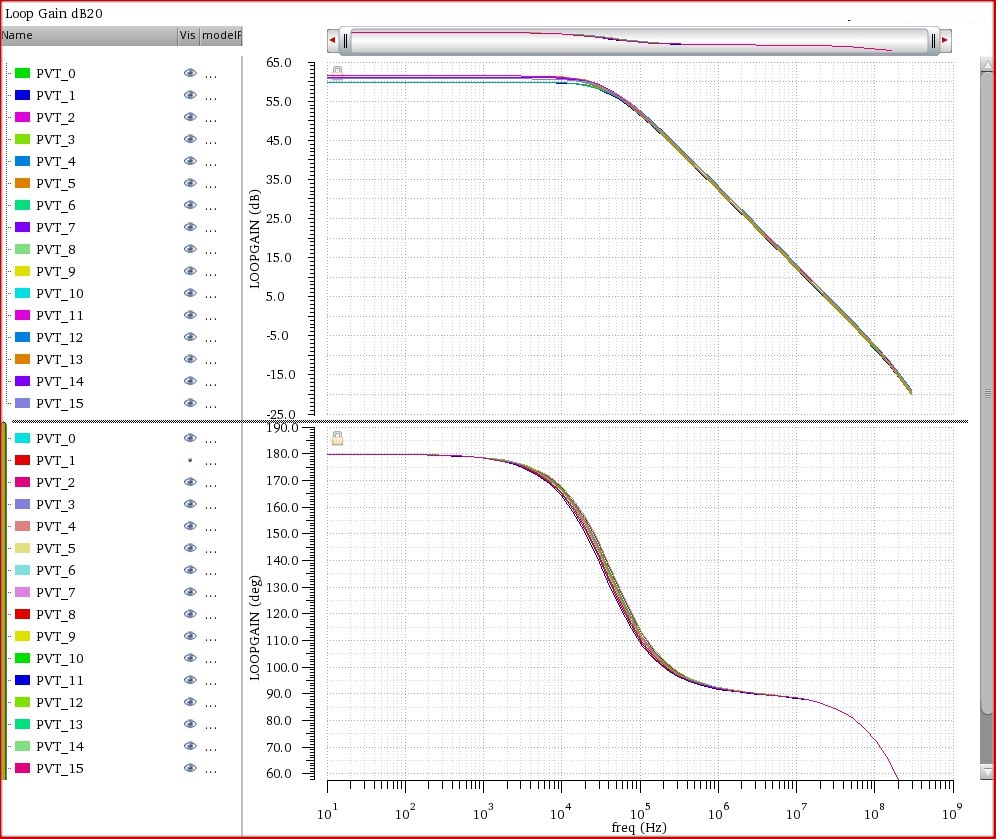
\includegraphics[width=\textwidth]{images/corner_gbw_phase_1.jpg}
\caption{Corner simulation of the OTA 1 frequency response}
\label{corner_freq_1}
\end{figure}

\begin{figure}[H]
\centering
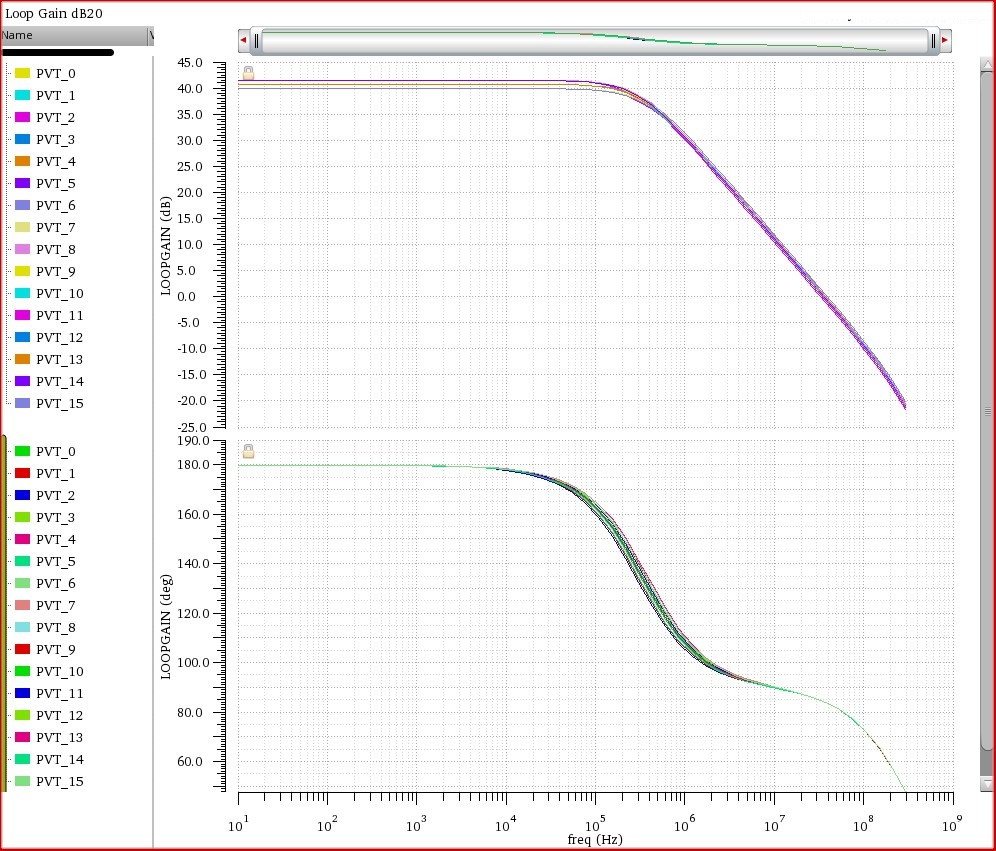
\includegraphics[width=\textwidth]{images/corner_gbw_phase_2.jpg}
\caption{Corner simulation of the OTA 2 frequency response}
\label{corner_freq_2}
\end{figure}


\begin{figure}[H]
\centering
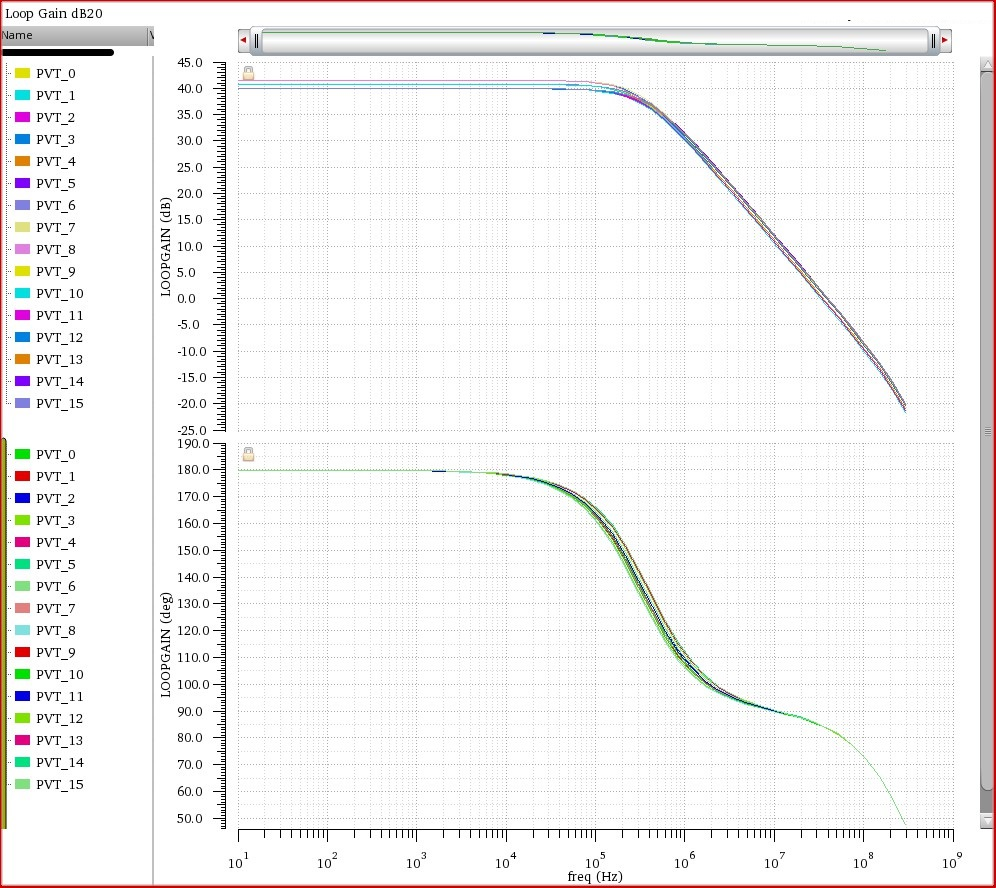
\includegraphics[width=\textwidth]{images/corner_gbw_phase_3.jpg}
\caption{Corner simulation of the OTA 3 frequency response}
\label{corner_freq_3}
\end{figure}

The slew rates for all corners for OTA 1, 2 and 3 are depicted in figures \ref{corner_slew_1}, \ref{corner_slew_2} and \ref{corner_slew_3}, and all have worst case in corner 5. With slew rates of 36.9MV/sec, 40.3MV/sec and 38.9MV/sec one can ensure a good enough settling time with good margin. 

\begin{figure}[H]
\centering
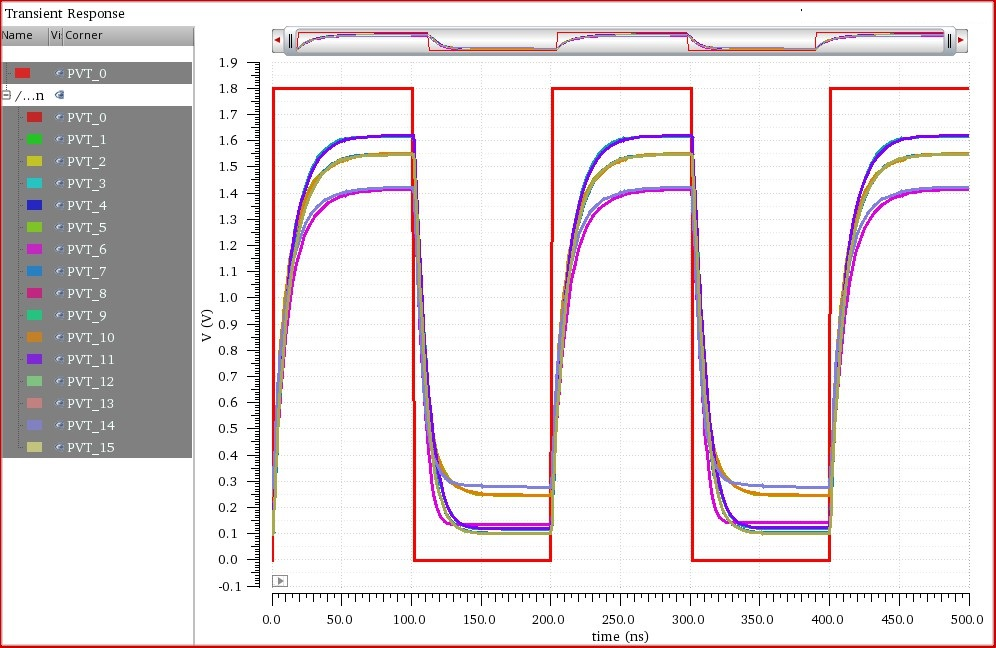
\includegraphics[width=\textwidth]{images/corner_slew_rate_1.jpg}
\caption{Corner simulation of the OTA 1 slew rate}
\label{corner_slew_1}
\end{figure}

\begin{figure}[H]
\centering
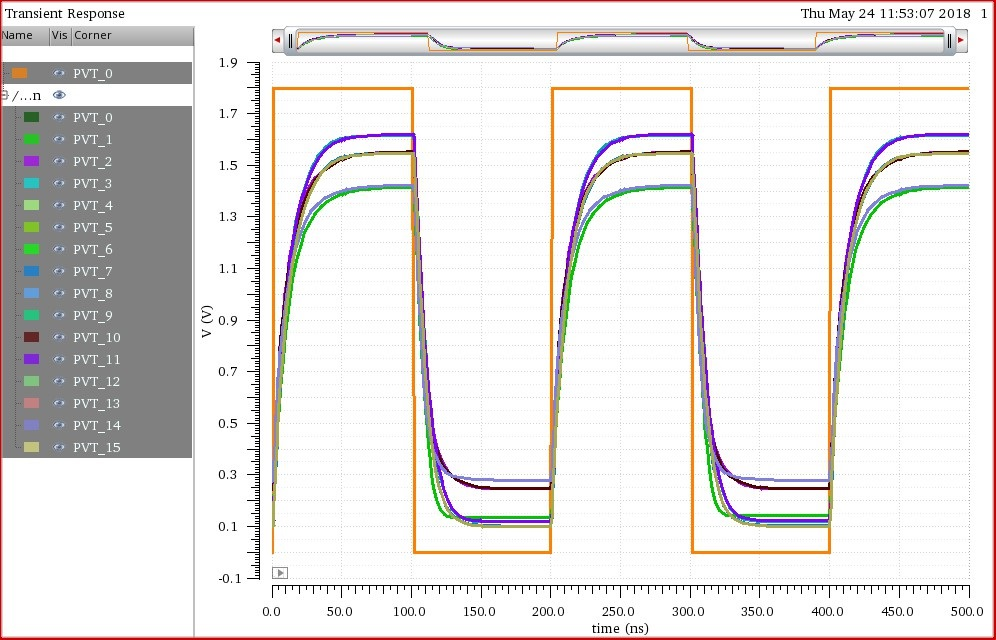
\includegraphics[width=\textwidth]{images/corner_slew_rate_2.jpg}
\caption{Corner simulation of the OTA 2 slew rate}
\label{corner_slew_2}
\end{figure}

\begin{figure}[H]
\centering
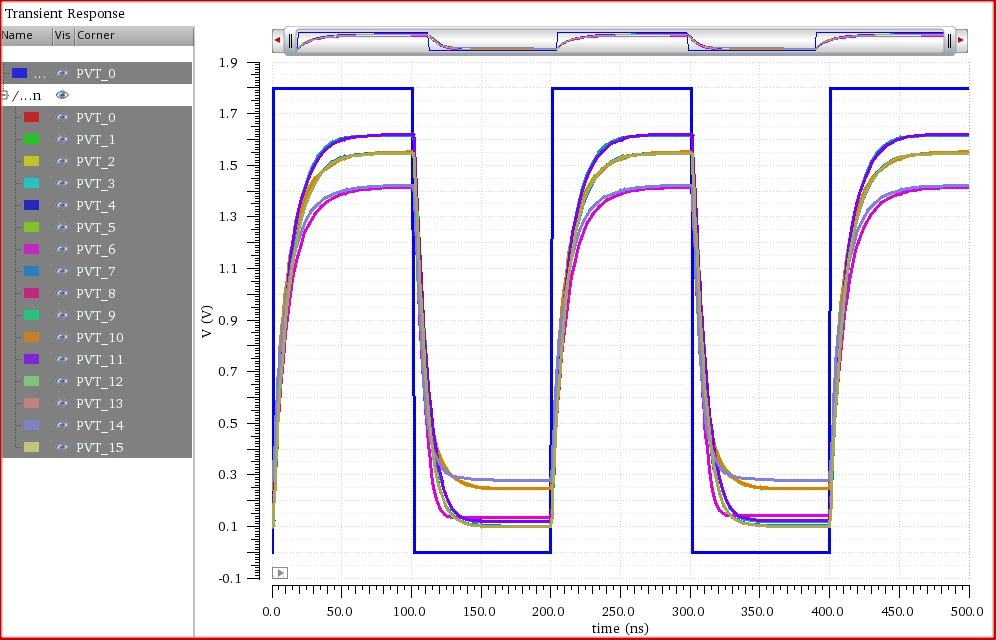
\includegraphics[width=\textwidth]{images/corner_slew_rate_3.jpg}
\caption{Corner simulation of the OTA 3 slew rate}
\label{corner_slew_3}
\end{figure}

\section{Modulator}
The response of the modulator was validated using nominal and PVT simulations with the corners listed in table \ref{corners}. A Noiseless and noisy simulations were simulated to confirm that the specification given by the thesis is achieved.  

\subsection{Noiseless simulations}
The modulator was simulates using transient analysis without imposing device noise. Nominal simulation was simulated, and the PSD of the output signal is shown in Fig \ref{psd_out}. The modulator achive a SNR of 101.20dB, a SINAD of 100.11dB and a ENOB of 16.5 bits. Here the only noise source is produced by the quantizer. 

Table \ref{modul_noiseless_out} summarize the SNRs, SINADs and ENOBs for all sixteen corners. It can be observed that all the corners fulfill the requirement of 16 bits, with corner 12 producing the lowest. Note that corner 12 is one of the corners with the lowest power consumption. 

\begin{figure}[H]
\centering
\includegraphics[width=\textwidth]{images/psd_out.jpg}
\caption{Nominal PSD of the modulator }
\label{psd_out}
\end{figure}

\begin{table}[H]
\centering

\caption{Results of the PVT simulations of the noiseless modulator}
\label{modul_noiseless_out}
\begin{tabular}{l|l|l|l}
\hline
\multirow{1}{*}{Simulation} & \multicolumn{1}{c|}{SINAD[dB]} & \multicolumn{1}{c|}{SNR[dB]} & \multicolumn{1}{c}{ENOB[bits]} \\\cline{1-4}
                       
            Nominal       &100.11 & 101.20 & 16.5\\
            Corner 0      &97.52 & 99.71 & 16.2\\
            Corner 1      &99.12 & 100.62 & 16.3\\
            Corner 2      &101.22 & 101.50 & 16.6\\
            Corner 3     &101.95 & 102.90 & 16.8\\
            Corner 4     &98.83 & 100.31 & 16.3\\
            Corner 5      &100.46 & 101.91 & 16.6\\
            Corner 6      &101.45& 101.83 & 16.6\\
            Corner 7      &100.78& 101.32 & 16.5\\
            Corner 8      &99.39& 100.84 & 16.4\\
            Corner 9      &101.94& 102.19 & 16.7\\
            Corner 10      &99.89& 101.43 & 16.6\\
            Corner 11      &101.86& 102.31 & 16.7\\
            Corner 12      &96.29& 97.30 & 16.1\\
            Corner 13      &98.54& 99.62 & 16.2\\
            Corner 14      &100.67& 101.44 & 16.5\\
            Corner 15      &100.74& 101.61 & 16.5\\
            
\hline            
\end{tabular}
\end{table}

\subsection{Noise simulation}
The modulator was simulated transient noise feature of the simulator. The PSD of the output signal is depicted in Fig \ref{psd_noise_out}. The PVT simulations are listed in table \ref{modul_noisy_out} where it can be observed that all corners except corners 0 and 12 achieve the specification of 16 bit. Nonetheless this is not a big problem as it is expected when introducing noise. Furthermore 15.7 and 15.8 bits are quite close to 16 bits. 

\begin{figure}[H]
\centering
\includegraphics[width=\textwidth]{images/psd_noise_out.jpg}
\caption{Nominal noisy PSD of the modulator output }
\label{psd_noise_out}
\end{figure}

\begin{table}[H]
\centering

\caption{Results of the PVT simulations of the noisy modulator}
\label{modul_noisy_out}
\begin{tabular}{l|l|l|l}
\hline
\multirow{1}{*}{Simulation} & \multicolumn{1}{c|}{SINAD[dB]} & \multicolumn{1}{c|}{SNR[dB]} & \multicolumn{1}{c}{ENOB[bits]} \\\cline{1-4}
                       
            Nominal      &98.23 & 99.67 & 16.2\\
            Corner 0      &93.65 & 94.86 & 15.8\\
            Corner 1      &95.78 & 96.31 & 16.0\\
            Corner 2      &98.93 & 100.54 & 16.3\\
            Corner 3     &100.76 & 101.12 & 16.4\\
            Corner 4     &96.59 & 97.23 & 16.1\\
            Corner 5      &99.41 & 100.73 & 16.3\\
            Corner 6      &96.78 & 97.20 & 16.1\\
            Corner 7      &98.26 & 99.75 & 16.2\\
            Corner 8      &95.84 & 96.44 & 16.0\\
            Corner 9      &100.77 & 101.34 & 16.5\\
            Corner 10      &99.00 & 100.75 & 16.4\\
            Corner 11      &100.78 & 101.55 & 16.6\\
            Corner 12      &93.89 & 94.2 & 15.7\\
            Corner 13      &95.55 & 96.15 & 16\\
            Corner 14      &96.69 & 97.23 & 16.1\\
            Corner 15      &98.76 & 99.9 & 16.3\\
            
\hline            
\end{tabular}
\end{table}


\section{Summary of the performance }
Tables \ref{comparsion_works} and \ref{comparsion_works_2} summarize the main results\footnote{Main results from nominal simulation with transient noise.} and compare it with similar works. It can be seen that the figure of merit (FoM)\footnote{$FoM = \frac{P}{2^{ENOB}\cdot2f_b}[\frac{pJ}{step}]$} is not the lowest, but it has the potential to get smaller by using techniques to reduce the power consumption. However, it seems to stand the ground with other works using 0.18$\mu m$ CMOS process. 


\begin{table}[H]
\centering
\caption{Comparison with other works}
\label{comparsion_works}
\begin{tabular}{l|l|l|l|l|l}
\hline
\multirow{1}{*}{Ref.} & \multicolumn{1}{c|}{Process [$\mu$m]} & \multicolumn{1}{c|}{OSR} & \multicolumn{1}{c|}{fs [MHz]} & \multicolumn{1}{c|}{Supply [V]} & \multicolumn{1}{c}{BW [kHz]}  \\\cline{1-6}

            \cite{ref_1} & 1.5 & 64 & 10.24 & 5 & 160\\
            \cite{ref_2} & 3 & 256 & 4 & 5 & 8\\
            \cite{ref_3} & 0.35 & 256 & 12.8 & 3.3 & 25\\
            \cite{SQNR} & 0.18 & 256 & 1 & 1.8 & 2 \\
            \cite{ref_4} & 0.18 & 128 & 0.256 & 1.5 & 1.0\\ 
            \cite{ref_5} & 0.13 & 40 & 1.048 & 1 & 8.0 \\
            \cite{ref_6} & 0.18 & 256 & 5.12 & 3.3 & 10\\
            \cite{ref_7} & 0.18 & 250 & 5 & 1.8 & 10\\
            \cite{ref_8} & 0.18 & 64 & 1.28 & 1.8 & 10\\
            \cite{ref_9} & 0.13 & 40 & 0.8& 0.8& 10 \\
            This work & 0.18 & 170 & 10 & 1.8 & 29\\

\hline            
\end{tabular}
\end{table}


\begin{table}[H]
\centering

\caption{Comparison with other works continued}
\label{comparsion_works_2}
\begin{tabular}{l|l|l|l|l}
\hline
\multirow{1}{*}{Ref.} & \multicolumn{1}{c|}{Power [$\mu$W]} & \multicolumn{1}{c|}{SINAD [dB]} & \multicolumn{1}{c|}{ENOB [bit]} & \multicolumn{1}{c}{FoM [pJ/step]}\\\cline{1-5}

        \cite{ref_1} & 7600 & 91 & 16 & 0.37\\
        \cite{ref_2} &  1200 & 89 & 14.5 & 3.24\\
        \cite{ref_3} & 6600 & 82 & 14 & 16.11\\
        \cite{SQNR} & 61 & 102.1 & 16.7 & 0.14\\
        \cite{ref_4} & 1350 & 93 & 15.2 & 18.49 \\
        \cite{ref_5} & 38.0 & 92 & 15.0 & 0.07 \\
        \cite{ref_6} & 1630 & 99 & 16.2 & 1.12\\
        \cite{ref_7} & 83 & 84.7 & 15 & 0.13\\
        \cite{ref_8} & 210 & 95 & 15.5 & 0.23\\
        \cite{ref_9} & 48 & 82 & 13.3 & 0.23\\
        This work & 87 & 98.2 & 16.2 & 0.20\\
\hline            
\end{tabular}
\end{table}
\chapter{Conclusion}




% Bibliography - edit references.bib and use the \cite command in text
\bibliographystyle{plain}
\bibliography{references}

\begin{thebibliography}{9}

\bibitem{Richard}
R. Schreier and G. C. Temes,
\textit{"Understanding Delta-Sigma Data Converters"},
New York,
IEEE press,
Wiley-Interscience,
ISBN:0-471-46585-2,
2005,

\bibitem{for_pro}
Duvarahan K. \textit{Design and Behavioral Modeling of a High Resolution, Discrete-Time Delta-Sigma ADC }, NTNU, 2017

\bibitem{Ovi}
Ovidiu B, Johan H.h, 
\textit{"Systematic Design of Sigma-Delta A/D Converters"},
Kluwer Academic Publishers,
ISBN: 1-4020-7945-1

\bibitem{Allen}
Allen P.E,  Holberg D.R, 
\textit{"CMOS Analog Circuit Design"},
Oxford University press,
ISBN: 0-19-51 1644-5

\bibitem{Johns}
Johns D.A, Martin K, 
\textit{"Analog Integrated Circuit Design"},
John Wiley and Sons inc. ,
ISBN: 984-12-647-0

\bibitem{Razavi}
Razavi B, 
\textit{"Principles of Data Conversion System Design"}, 
IEEE press,
ISBN : 0-7803-1093-4

\bibitem{Barker}
Barker J.R,
\textit{"CMOS Mixed-Signal Circuit Design" },
IEEE press
ISBN: 0-471-22754-4

\bibitem{deltapic}
M.Ortmanns and F.Gerfers,
\textit{"Continuous-Time Sigma-Delta A/D Conversion
Fundamentals,PerformanceLimits and Robust Implementations"},
Secaucus,
NJ,USA:
Springer-Verlag
NewYork,
Inc.,
ISBN:978-3-540-28406-2.
Springer Series in Advanced Micro electronics
Volume21,
2006.

\bibitem{charge_pump}
B.R. Gregoire,
\textit{A switched capacitor regulated charge pump power supply},
Custom Integrated Circuits Conference, 2005, Proceedings of the IEEE 2005,
ISBN: 0-7803-9 023-7

\bibitem{SQNR}
J. V. De la C. Marin,
\textit{INTEGRATED CIRCUIT DESIGN OF SIGMA-DELTA MODULATOR FOR
ELECTRIC ENERGY MEASUREMENT APPLICATIONS},
instituto alberto luiz coimbra de pós-graduação e pesquisa de engenharia,
RIO DE JANEIRO, RJ – BRASIL,
2013

\bibitem{William}
Schweber, William L.,
\textit{Integrated Circuits for Computers: Principles and Applications},
McGraw-Hill, pp. 157-158,
ISBN: 978-0-070-53624-1

\bibitem{Malo}
Maloberti F, 
\textit{"Data Converters"}
Dordrecht, Netherlands,
Springer 2007,
ISBN: 978-0387324852.

\bibitem{load}
Jian X, Hanqing W, Xiaobo W,
\textit{A 20 micro 95dB DR Single-Bit Delta-Sigma Modulator for Portable Measurement Applications},
Proceedings of the international MultiConference of Engineers and Computer Scientists 2010 Vol 2,
IMECS 2010, March 17-19, 2010, Hong Kong

\bibitem{gm_id_1}
F.Silveira, D.Flandre and P.G.A Jespers
\textit{A $g_m/I_D$ Based Methodology for the Design of CMOS Analog Circuits and Its application to the Synthesis of a Silicon-on-Insulator Micropower OTA},
IEEE journal of solid-state circuits, VOL. 31 NO. 9 September 1996.


\bibitem{first_delta}
H.Inose, Y.Yasuda and J.Murakami,
\textit{"A Telemetry System by Code Modulation - Delta-Sigma Modulation"},
Space Electronics and Telemetry,
IRE Transactions on vol.
SET-8, pp. 204-209,
1962

\bibitem{two_stage_1}
Rio.F, R.Mederio Hidalgo, F. Perez-Verdu, B. Rosa Ultrera, J.M. Rodriquez-Vazquez,
\textit{CMOS Cascade Sigma-Delta Modulators for Sensors and Telecom Error Analysis and Practical Design },
Springer Netherlands, 2006,
ISBN: 978-1-4020-4776-3

\bibitem{Plass}
Plassche R., 
\textit{"CMOS Integrated Analog-to-Digital and Digital-to-Analaog converters"},
Boston, Kluwer Academic Publisers, 2003,
ISBN: 978-3-540-28473-4

\bibitem{corr}
 C.C. Enz ; G.C. Temes,
 \textit{"Circuit techniques for reducing the effects of op-amp imperfections: autozeroing, correlated double sampling, and chopper stabilization"},
 Proceedings of the IEEE,
 vol 84, issue 11,
 pp. 1584-1614,
 1996

\bibitem{phase}
David F.S and Kaufman M, 
\textit{Handbook of operational amplifier circuit design},
NY: Mc-Graw-Hill,
Sec. 3-4, 
ISBN 0-07-061797-X

\bibitem{Lee}
K.-H. Chao, S.Nadeem, W.Lee and C.Sodini, 
\textit{"A higher order topology for interpolative modulators for oversampling A/D converters"},
Circuits and Systems, IEEE Transactions on, vol. 37, pp. 309-318 mar 1990.

\bibitem{cds}
W. H. White, D. R. Lampe, F. C. Blaha, and 1. A. Mack, \textit{“Characterization
of surface channel CCDimage arrays at low light levels"}
IEEE J. Solid-State Circuits, vol. SC-9, pp. 1-14, Feb. 1974.

\bibitem{private}
Private communication with \textit{Microchip}.

\bibitem{Grey}
P. R. Grey, P. J. Hurst, S. H. Lewis, R. Meyer,
\textit{Analysis and Design of Analog Integrated Circuits},
John Wiley Sons, 5th edition 2009,
ISBN: 978-0470245996


\bibitem{two_stage_2}
Yao I., Steyaert M., Sansen W., 
\textit{Low-power low-voltage sigma-delta modulators in nanometer CMOS},
Springer Netherlands, 2006,
ISBN: 978-1-4020-4140-2

\bibitem{gm_id_2}
H.D. Danmark, S.Bensalem, S.Zouari and M.Loulou
\textit{Design of Folded Cascode OTA in Different Regions of Operation though $g_m/I_D$ Methodology},
World Academy of Science, Engineering and Technology International Journal of Electrical and Computer Engineering, Vol. 2, No. 9, 2008

\bibitem{ref_1}
Mike.R, Nicholas R.V.B, Patrick R, Robert G, James C, John R.H,
\textit{A 16-b 160-kHz CMOS A/D Converter Using Sigma-Delta Modulation},
IEEE Journal of Solid-State Circuits, VOL 25, Issue 2, April 1990, pp. 431-440.

\bibitem{tool}
R.Schreier,
\textit{Delta-Sigma Toolbox},
2010
[Online]
Avaliable:
\url{http:www.mathworks.com/matlabcentral/fileexchange/19}.

\bibitem{comparator}
Ho J, Luong H,
\textit{A 3-V 1.47mW 120MHz Comparator for Use in Pipline ADC},
Proceedings of IEEE Asia-Pacific Conference on Circuits and System 96, p. 413-416, November 1996

\bibitem{adaptive}
Antonio J.L.M, Sushmita B, Jaime R.A, Ramon G.C,
\textit{Low-Voltage Super CLass AB CMOS OTA Cells With Very High Slew Rate and Power Efficiency},
IEEE J. Solid-State Circuits, vol 40 no 5, pp. 1068-1077, October 2005.

\bibitem{ref_2}
Bernhard E.B, Bruce A.W,
\textit{The Design of Sigma-Delta Modulation Analog-to-Digital Converters},
IEEE, Journal of Solid-State Circuits, VOL 23, NO 6, December 1998, pp. 1298-1308.

\bibitem{ref_3}
Sumit K.N, 
\textit{Design of a 14-bit fully differential discrete time delta-sigma modulator},
Rochester Institute of Technology, RIT Scholar works, 11.15.2006.
\bibitem{ref_4}
Yongsheng W, Yuanhong L, Mingyan Y.,
\textit{A 16 bit low voltage low power Delta Sigma modulator}.
Proceedings of 2011 International Conference on Electronics and Mechanical Engineering and Information Technology, VOL 6, pp. 3178-3181, 2011.

\bibitem{ref_5}
Da Q., Yuan-wen L., Long C., Jun X., Fan Y., Jun-yan R.,
\textit{An ultra low power sigma-delta modulator for hearing aid double-sampling},
IEEE, 8th International Conference on ASIC, pp. 1141-1144, 2009.

\bibitem{ref_6}
Zhijun L., Benoit G., Mohamad S., 
\textit{A 16-bit sigma-delta modulator for low power medical implantable sensors}
IEEE, International Conference on Electronics, Circuits and System, pp. 1-4, 2005

\bibitem{ref_7}
Joshua L., DAvid A. J., 
\textit{A frequency-scalable 15-bit incremental ADC for low power sensor applications},
IEEE, International Symposium on Circuits and System, pp. 2418-2421, 2010.

\bibitem{ref_8}
Serena P., Francesco C. Chris V. H., Eugenio C., Arthur H. M. van R., 
\textit{A Power-Optimal Design Methodology for High-Resolution Low-Bandwidth SC Delta-sigma Modulators},
IEEE Transactions on Instrumentation and Measurement, VOL. 61, Issue. 11, pp. 2896-2904, 2012

\bibitem{ref_9}
Wei L., Peiyuan W., Pingfen L.,
\textit{A 0.8-V 48uW 82dB SNDR 10-kHz bandwidth delta-sigma modulator},
IEEE, international Symposium, pp. 89-91, 2012
\end{thebibliography}


\begin{appendices}

\chapter{Switch transistors' dimensions and resistance}
\label{app:on_resistance}

\section{Integrator 2}
\label{app:int_2_on}

\begin{table}[H]
\centering
\caption{Switch transistors' dimensions and resistances of integrator 2}
\label{R_on_2}
\begin{tabular}{|l|l|l|l|}
\hline
Switch & PMOS( W/L)$\mu m$ & NMOS( W/L)$\mu m$ & $R_{ON} (\Omega)$   \\ \hline
I15    & 9.3/0.55  & 3.1/0.55   & 1493 \\ \hline
I17     & 9/0.55  & 3/0.55   & 1531 \\ \hline
I21    & 7.8/0.55  & 2.6/0.55   & 1530 \\ \hline
\end{tabular}
\end{table}

\section{Integrator 3}
\label{app:R_on_3}
\begin{table}[H]
\centering
\caption{Switch transistors' dimensions and resistances of integrator 3}
\label{R_on_3}
\begin{tabular}{|l|l|l|l|}
\hline
Switch & PMOS( W/L)$\mu m$ & NMOS( W/L)$\mu m$ & $R_{ON} (\Omega)$   \\ \hline
I15    & 7.8/0.55  & 2.6/0.55   & 1635 \\ \hline
I21     & 7.9/0.55  & 2.63/0.55   & 1630 \\ \hline
\end{tabular}
\end{table}

\section{Sum Block}
\label{app:sum_block_on}

\begin{table}[H]
\centering
\caption{Switch transistors' dimensions and resistances of sum block}
\label{R_on_sum}
\begin{tabular}{|l|l|l|l|}
\hline
Switch & PMOS( W/L)$\mu m$ & NMOS( W/L)$\mu m$ & $R_{ON} (\Omega)$   \\ \hline
I7    & 7.2/0.55  & 2.4/0.55   & 1700 \\ \hline
I5     & 8.1/0.55  & 2.7/0.55   & 1701 \\ \hline
I4    & 9/0.55  & 3/0.55   & 1705 \\ \hline
I3    & 7.8/0.55  & 2.6/0.55   & 1743 \\ \hline
I35    & 6.6/0.55  & 2.2/0.55   & 1706 \\ \hline
\end{tabular}
\end{table}

\chapter{Circuits}\label{app:cicuits}

\section{Integrator 1}
\label{app:integrator_1}
\begin{center}
\includegraphics[width=\textwidth]{images/Integrator_1.png}
\end{center}

\section{Remaining integrators}
\label{app:integrator_rest}
\begin{center}
\includegraphics[width=\textwidth]{images/integrator_2.png}
\end{center}

\section{Summation node}
\label{app:sum}
\begin{center}
\includegraphics[width=\textwidth]{images/sum_block.png}
\end{center}

\section{Top module}
\label{app:top}
\begin{center}
\includegraphics[width=\textwidth]{images/top_module.png}
\end{center}

\section{SR latch circuit}
\label{app:SR}
\begin{center}
\includegraphics[width=\textwidth]{images/SR_latch_block.png}
\end{center}

\end{appendices}




\end{document}
